\documentclass[12pt,a4paper,uplatex]{jsbook}
\usepackage[utf8]{inputenc}
%\usepackage{graphicx}
%\usepackage{bm}
%\usepackage{amsmath}

\usepackage[T1]{fontenc}
\usepackage{ascmac, here, txfonts, txfonts}
\usepackage{listings, jlisting}
\usepackage{color}
\usepackage{fancybox}
\usepackage{comment}
\usepackage[dvipdfmx]{graphicx}
\usepackage {colortbl,array,xcolor}
\usepackage{framed}
\usepackage {boites}
\usepackage{eclbkbox}
\usepackage[hyphens]{url}
\usepackage{here}
\usepackage{setspace}
%\usepackage{listings,jlisting} %日本語のコメントアウトをする場合jlistingが必要
\begin{comment}
%ここからソースコードの表示に関する設定
%\lstset{
	%  basicstyle={\ttfamily},
	%  identifierstyle={\small},
	%  commentstyle={\smallitshape},
	%  keywordstyle={\small\bfseries},
	%  ndkeywordstyle={\small},
	%  stringstyle={\small\ttfamily},
	%  frame={tb},
	%  breaklines=true,
	%  columns=[l]{fullflexible},
	%  numbers=left,
	%  xrightmargin=0zw,
	%  xleftmargin=3zw,
	%  numberstyle={\scriptsize},
	%  stepnumber=1,
	%  numbersep=1zw,
	%  lineskip=-0.5ex
	%}
\lstset{
	basicstyle={\ttfamily},
	identifierstyle={\small},
	commentstyle={\smallitshape},
	keywordstyle={\small\bfseries},
	ndkeywordstyle={\small},
	stringstyle={\small\ttfamily},
	frame={tb},
	breaklines=true,
	columns=[l]{fullflexible},
	numbers=left,
	xrightmargin=0zw,
	xleftmargin=3zw,
	numberstyle={\scriptsize},
	stepnumber=1,
	numbersep=1zw,
	lineskip=-0.5ex
}
%ここまでソースコードの表示に関する設定
\makeatletter
\def\ps@plainfoot{%
	\let\@mkboth\@gobbletwo
	\let\@oddhead\@empty
	\def\@oddfoot{\normalfont\hfil-- \thepage\ --\hfil}%
	\let\@evenhead\@empty
	\let\@evenfoot\@oddfoot}
\let\ps@plain\ps@plainfoot
\renewcommand{\chapter}{%
	\if@openright\cleardoublepage\else\clearpage\fi
	\global\@topnum\z@
	\secdef\@chapter\@schapter}
\makeatother
%
\newcommand{\maru}[1]{{\ooalign{%
			\hfil\hbox{$\bigcirc$}\hfil\crcr%
			\hfil\hbox{#1}\hfil}}}
%
\setlength{\textwidth}{\fullwidth}
\setlength{\textheight}{40\baselineskip}
\addtolength{\textheight}{\topskip}
\setlength{\voffset}{-0.55in}
%
\end{comment}
\lstset{
	%プログラム言語(複数の言語に対応,C,C++も可)
	language = Python,
	%背景色と透過度
	backgroundcolor={\color[gray]{.90}},
	%枠外に行った時の自動改行
	breaklines = true,
	%自動改行後のインデント量(デフォルトでは20[pt])	
	breakindent = 10pt,
	%標準の書体
	basicstyle = \ttfamily\scriptsize,
	%コメントの書体
	commentstyle = {\itshape \color[cmyk]{1,0.4,1,0}},
	%関数名等の色の設定
	classoffset = 0,
	%キーワード(int, ifなど)の書体
	keywordstyle = {\bfseries \color[cmyk]{0,1,0,0}},
	%表示する文字の書体
	stringstyle = {\ttfamily \color[rgb]{0,0,1}},
	%枠 "t"は上に線を記載, "T"は上に二重線を記載
	%他オプション:leftline,topline,bottomline,lines,single,shadowbox
	frame = TBrl,
	%frameまでの間隔(行番号とプログラムの間)
	framesep = 5pt,
	%行番号の位置
	numbers = left,
	%行番号の間隔
	stepnumber = 1,
	%行番号の書体
	numberstyle = \tiny,
	%タブの大きさ
	tabsize = 4,
	%キャプションの場所("tb"ならば上下両方に記載)
	captionpos = t
}
\begin{comment}
\lstset{
	%プログラム言語(複数の言語に対応,C,C++も可)
	language = Java,
	%背景色と透過度
	backgroundcolor={\color[gray]{.90}},
	%枠外に行った時の自動改行
	breaklines = true,
	%自動改行後のインデント量(デフォルトでは20[pt])	
	breakindent = 12pt,
	%標準の書体
	basicstyle = \ttfamily\scriptsize,
	%コメントの書体
	commentstyle = {\itshape \color[cmyk]{1,0.4,1,0}},
	%関数名等の色の設定
	classoffset = 0,
	%キーワード(int, ifなど)の書体
	keywordstyle = {\bfseries \color[cmyk]{0,1,0,0}},
	%表示する文字の書体
	stringstyle = {\ttfamily \color[rgb]{0,0,1}},
	%枠 "t"は上に線を記載, "T"は上に二重線を記載
	%他オプション:leftline,topline,bottomline,lines,single,shadowbox
	frame = TBrl,
	%frameまでの間隔(行番号とプログラムの間)
	framesep = 5pt,
	%行番号の位置
	numbers = left,
	%行番号の間隔
	stepnumber = 1,
	%行番号の書体
	numberstyle = \tiny,
	%タブの大きさ
	tabsize = 4,
	%キャプションの場所("tb"ならば上下両方に記載)
	captionpos = none
}
\end{comment}

\renewcommand{\lstlistingname}{}

\setcounter{secnumdepth}{6}
\setcounter{secnumdepth}{6}

% Title Page
\title{Remote Sensor Project}
\author{S.Matoike}

\begin{document}

\maketitle
\tableofcontents

%\begin{abstract}
%\end{abstract}
\chapter{システム全体の概要}

\section{全体の構成}

\begin{figure}[H]
	\begin{minipage}[b]{1.0\linewidth}
		\centering
		\includegraphics[keepaspectratio, scale=0.5]{figs/eps/zentai.eps}
		\caption{システム全体の構成}
	\end{minipage}
	%	\hspace{1.0cm}
	%	\begin{minipage}[b]{0.45\linewidth}
		%		\centering
		%		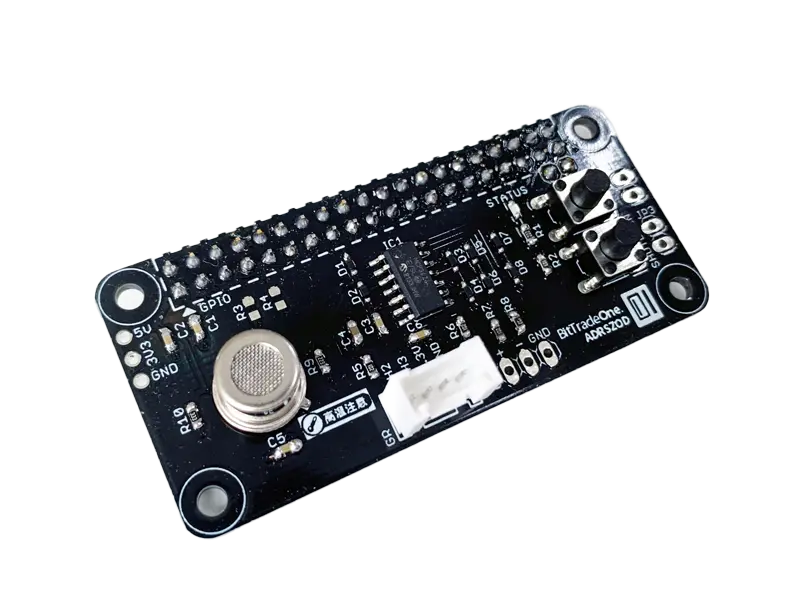
\includegraphics[keepaspectratio, scale=0.25]{figs/png/nioi_sensor.png}
		%		\caption{ADRSZOD:TP401A}
		%	\end{minipage}
\end{figure}

\begin{itemize}
	\item 5分毎にリモートマシン上の臭気センサの測定データをローカルマシンに読み取る
	\item 読み取った5分毎のデータは、追記、蓄積していくと同時に、実時間の臭気変化としてグラフを描画更新する(ローカルマシン上)
	\item 23時56分に、日毎の処理を起動し、1日分の蓄積データをグラフ化すると共に、蓄積した1日分のデータは別フォルダに退避する(ローカルマシン上)
	\item 日曜日の0時1分に、週毎の処理を起動し、その日から過去1週間分の蓄積データを読んでグラフ化する(ローカルマシン上)
	\item クラウドにデータを保持することで、補助記憶装置の負荷を低減させるやり方は第3章にて
	%\item ローカルマシン上に蓄積されたデータは、適切なタイミングでクラウド上のGCS(google-cloud-storage)へ退避させ、ローカルマシンの補助記憶容量を圧迫することがない様にする(第3章)
\end{itemize}


\chapter{ローカルにデータを保持する}

\begin{table}[h]
	\centering
	\caption{ここで使用するshellとプログラム}
	\label{tab:local}
	\begin{tabular}{llp{8.5cm}}
		\hline
		リモート & sensor.sh & 日付文字列とセンサーの読み取り値を並べて出力するshell \\
		リモート & adrsz0D.py & センサーを読むクラスの定義 \\
		リモート & procmain.py & センサーのインスタンス生成とセンサーの読取り \\
		ローカル & rsensor.sh & 5分間隔でcronに呼び出される. リモートの sensor.sh を起動して、結果をローカルの w.txt に追記蓄積する \\
		ローカル & daily.sh & 23時56分にcronにより起動される. 1日の蓄積データ w.txt のdata/フォルダへの退避とdaily.pyの起動\\
		ローカル & daily.py & data/フォルダ内の指定した日付の1日分のデータを読んでグラフを作図する \\
		ローカル & weekly.sh & 毎週日曜日の0時1分にcronにより起動される. weekly.pyを起動する \\
		ローカル & weekly.py & data/フォルダ内の指定日より前の1週間分のデータを読んでグラフを作図する \\
		ローカル & rtplot.sh & rtplot.py を起動する. デスクトップに置いてマウスクリックで起動させる \\
		ローカル & rtplot.py & w.txt を監視して、更新される度に実時間グラフを更新表示する \\
		ローカル & myplot.py & daily.py、weekly.py から共通に呼び出されるグラフ作図用の関数 \\  \hline
	\end{tabular}
\end{table}


\section{リモートマシンの処理}

\subsection{リモート機器、センサー}

\begin{figure}[H]
	\begin{minipage}[b]{0.45\linewidth}
		\centering
		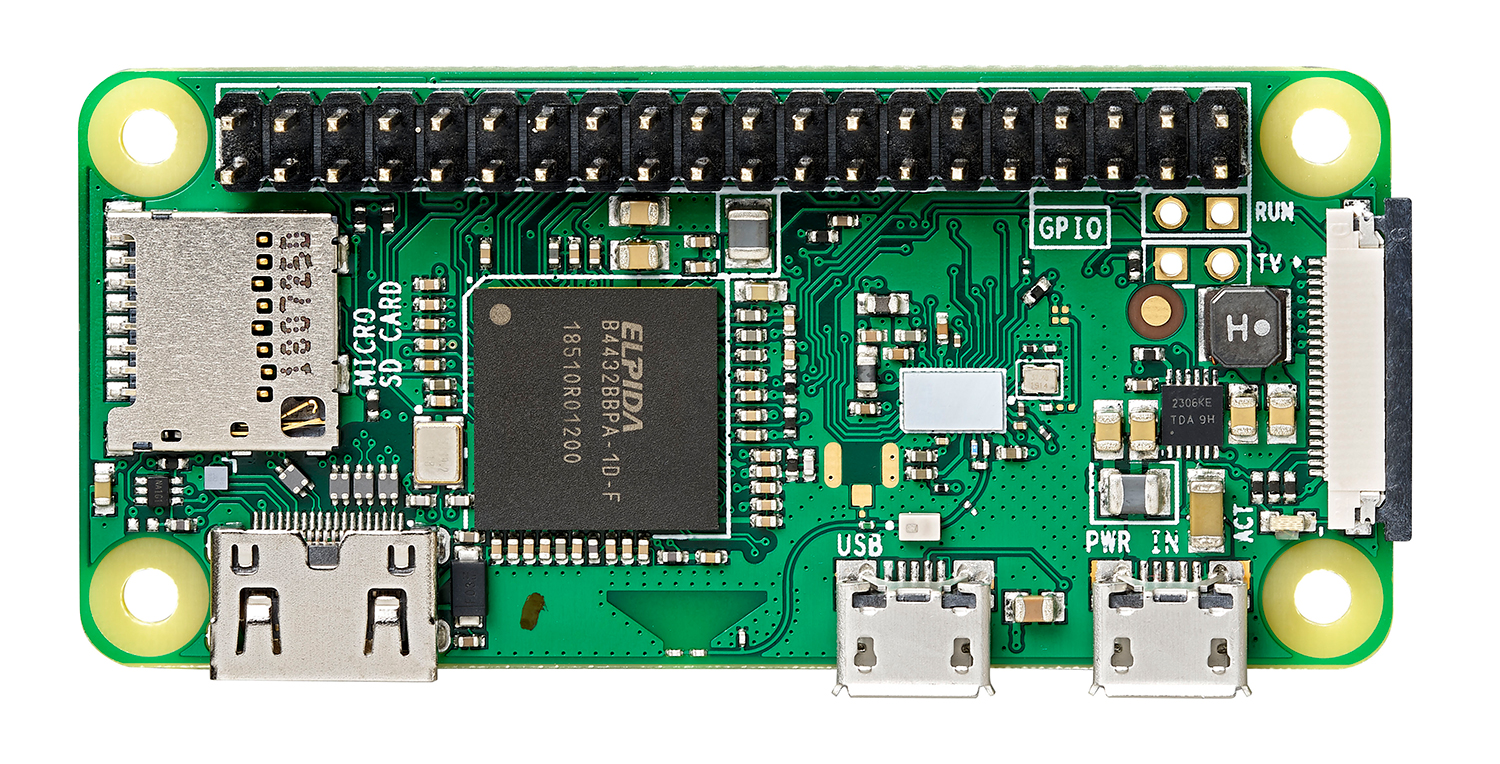
\includegraphics[keepaspectratio, scale=0.13]{figs/jpg/udrpzwh.jpg}
		\caption{Raspberry Pi Zero2 W / Zero W}
	\end{minipage}
	\hspace{1.0cm}
	\begin{minipage}[b]{0.45\linewidth}
		\centering
		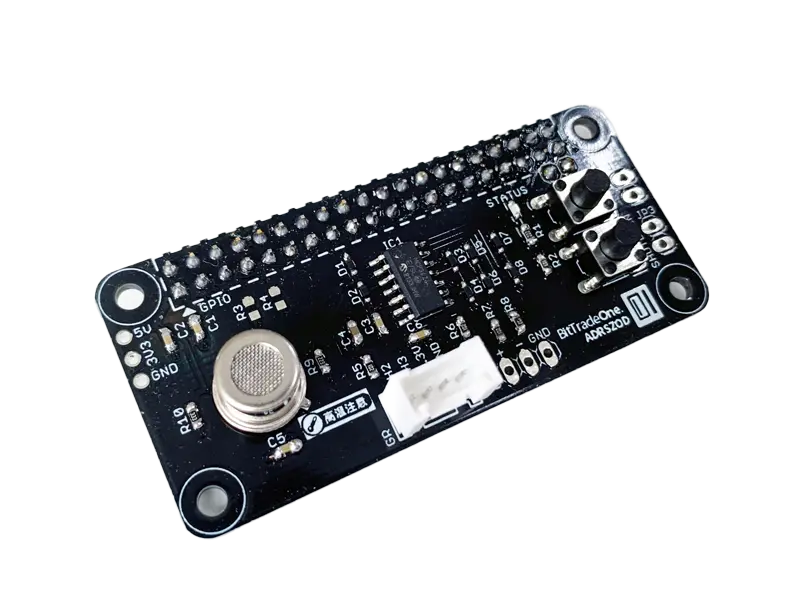
\includegraphics[keepaspectratio, scale=0.25]{figs/png/nioi_sensor.png}
		\caption{ADRSZOD:TP401A}
	\end{minipage}
\end{figure}

臭気センサTP-401A

\begin{itemize}
	\item 低電力で動作可能な高感度の臭気センサ
	\item コンパクトなRaspberry Pi Zero と重ねて使用可能な pHAT サイズ
	\item アンモニア、水素、アルコール、一酸化炭素、メタンなど揮発性気体、タバコ、木材燃焼発生した煙など様々な気体に対応
	\item 連続通電を許容するので、様々な所での継続的なチェックが可能(動作時にはセンサ部が非常に高温となるため、取り扱いには注意)
	\item 動作状況が見えるステータスLEDにより、駆動状況の確認が容易
\end{itemize}

%\newpage
運用方針

\begin{itemize}
	\item 基本的な運用形態は、モニタ、キーボード等を接続せず電源のみの接続で運用する
	\item このマシン上では、数行の shell を登録するだけなので、基本的には他のPCのコンソールから ssh でloginして利用する(ここの例では、ユーザは mat)
	\begin{verbatim}
		ssh mat@192.168.3.27
	\end{verbatim}
	\item VNCを有効にして他のPCからアクセスすれば、デスクトップも利用できる
\end{itemize}

\subsection{リモート処理の概要}

%\begin{itemize}
	Raspberrin Pi Zero2 W/Zero W  上に用意したこのshell(sensor.sh)は、別のRaspberryPiマシンからsshによって起動される
	
	I2Cで接続された臭気センサの出力(電圧値)は、Pythonのプログラム(adrszOD.py)によって読み取られる
	
	adrszOD.pyはAD変換器のch1からch4までの値を出力しているので、その出力をawkにパイプして、1つ目のch1の値だけを取り出している
	
	dateコマンドで作成している測定日付は、後ほどPythonのmatplotlibの都合に合わせて、新たにデータの整形処理が必要にならない様に、書式を「年−月−日と時:分:秒の間は、半角カンマ+半角スペース1個」の格好になる様に整形する
	
	日付とセンサの出力する値が1行になる様にするため、pasteコマンド(テキストファイルを横に並べて結合するコマンド)を使っている\footnotemark[1](shでは動かないので、bashにする)
	
	paste の2つのオペランド、<(date +....)と、<(python3 ..procmain.py..)の各々のコマンドは、<(any command) の形に囲むことにより、読み取りのためのファイル記述子を指定したことになり、それぞれを2つのファイルの様に扱うことができる\footnote[1]{「Efficient Linuxコマンドライン」オライリー・ジャパン 初版第1刷p.108、p.156(プロセス置換)}
%\end{itemize}

\begin{itembox}[l]{/home/mat/Documents/sensor.sh}
	\begin{verbatim}
#!/usr/bin/bash
dir='/home/mat/Documents'
paste <(date +%Y-%m-%d,\ %H:%M:%S) \
<(python3 ${dir}/procmain.py | awk '{print $1}')
	\end{verbatim}
\end{itembox}

この shell を起動してみると、次の通り

\begin{itembox}[l]{sensor.sh の出力例}
	\begin{verbatim}
mat@raspberrypizero:~/Documents $ ./sensor.sh 
2024-04-17, 02:40:55	ch1:0.79827
mat@raspberrypizero:~/Documents $ 
	\end{verbatim}
\end{itembox}

以下は、センサーを読むためのPythonのプログラム\footnote{\url{https://github.com/bit-trade-one/RasPi-Zero-One-Series}
}

\begin{spacing}{0.9}
\begin{itembox}[l]{/home/mat/Documents/adrszOD.py}
	\begin{verbatim}
import smbus, time

class I2C:
  i2c_bus = None
  def __init__(self, bus_number=1):
    cls = type(self)    # 旧スタイルなら、cls = self.__class__
    cls.i2c_bus = smbus.SMBus(bus_number) 

class TP401A(I2C):
  def __init__(self, address=0x68, Vref=2.048) -> None:
    super().__init__(bus_number=1)
    self.address = address
    self.Vref = Vref

  def swap16(self, x):
    return (((x << 8) & 0xFF00) | ((x >> 8) & 0x00FF))

  def sign16(self, x):
    return (-(x & 0b1000000000000000) | (x & 0b0111111111111111))

  def read_val(self, x):
    self.i2c_bus.write_byte(self.address, x) #16bit
    time.sleep(0.2)
    data = self.i2c_bus.read_word_data(self.address,0x00)
    raw = self.swap16(int(hex(data),16))
    raw_s = self.sign16(int(hex(raw),16))
    volts = round((self.Vref * raw_s / 32767),5)
    return volts
	\end{verbatim}
\end{itembox}
\end{spacing}

\newpage

クラスTP401Aが、クラスI2Cを継承する様にしたのは、新たな別のI2C対応デバイスを、同じバス上に接続する場合を想定したもの

TP401AクラスはI2Cクラスを継承しているので、TP401Aのコンストラクタの中でI2Cクラスのコンストラクタを明示的に実行し、I2Cバスの番号を指定している

TP401Aクラスの上位クラスI2Cクラスのクラス変数i2c\_busへのアクセスは、「self.変数名」の格好でアクセスすることによって、インスタンス変数→クラス変数→親クラスのクラス変数の順に探索され、I2Cクラスのクラス変数にたどり着けることになる

このTP401Aクラスを使う主処理は、sensor.sh の中から呼び出されている

\begin{itembox}[l]{/home/mat/Documents/procmain.py}
	\begin{verbatim}
#!/usr/bin/env python
from sarzOD import TP401A

if __name__  ==  "__main__":
  smel = TP401A()
  volts1 = smel.read_val( 0b10011000 ) 
  volts2 = smel.read_val( 0b10111000 ) 
  volts3 = smel.read_val( 0b11011000 ) 
  volts4 = smel.read_val( 0b11111000 )
  out_msg = f"ch1:{volts1} ,ch2:{volts2},ch3:{volts3},ch4:{volts4}" 
  print(out_msg)
	\end{verbatim}
\end{itembox}

\section{ローカルマシンの処理}

\subsection{ローカル機器}

\begin{figure}[H]
	\begin{minipage}[b]{1.0\linewidth}
		\centering
		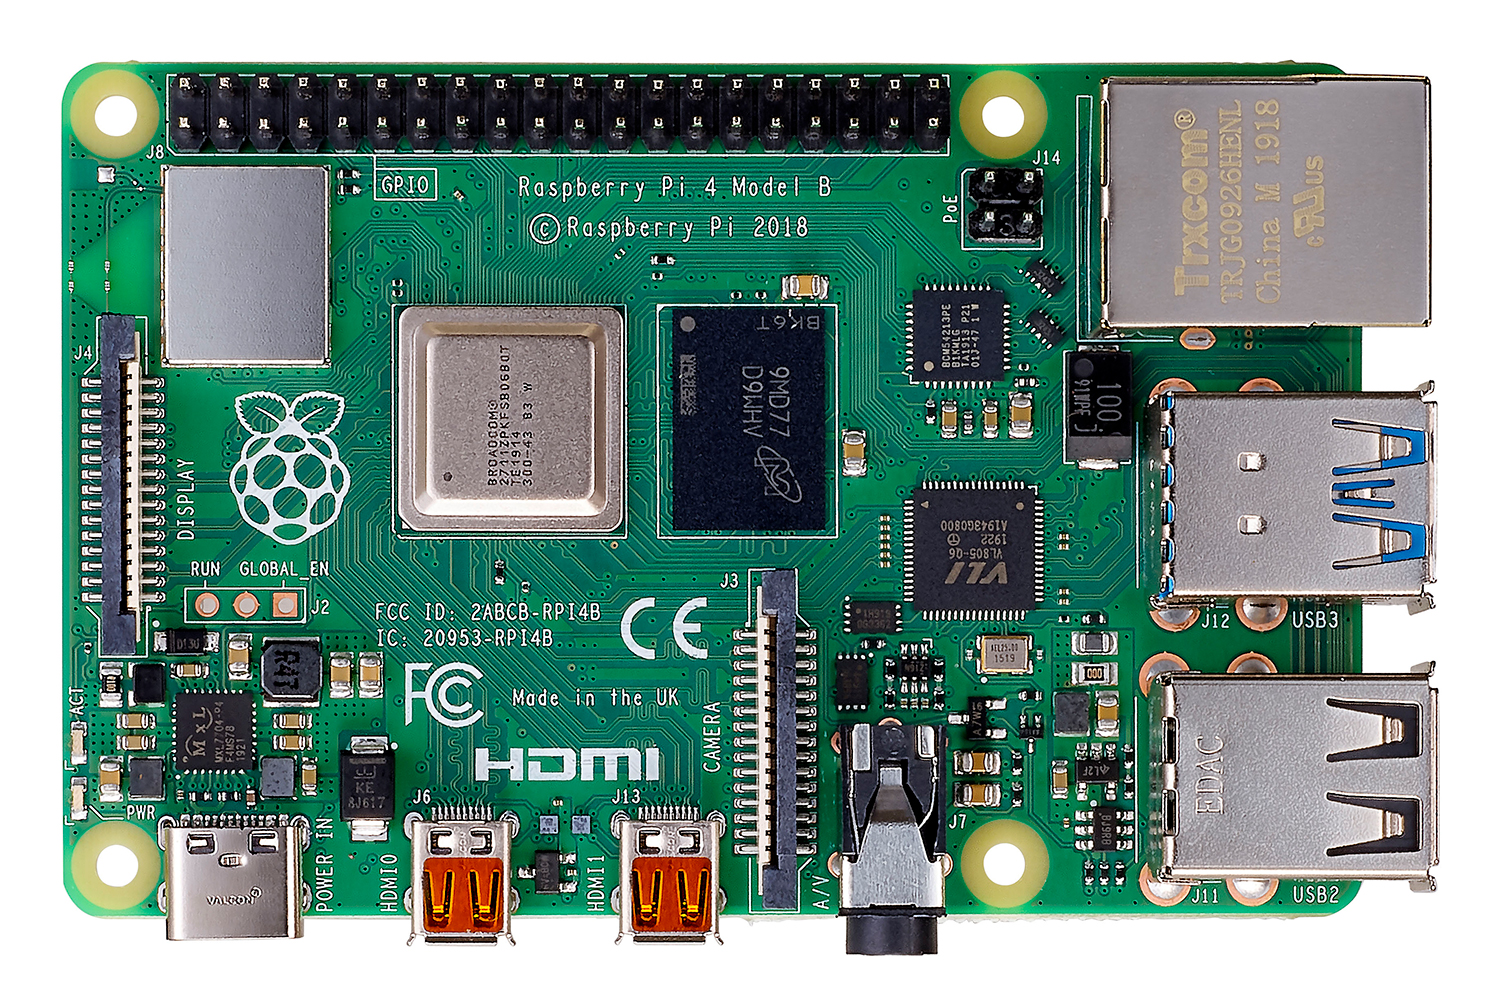
\includegraphics[keepaspectratio, scale=0.12]{figs/jpg/udrp4b_front.jpg}
		\caption{Raspberry Pi 3/4/5}
		%	\end{minipage}
	%	\hspace{1.0cm}
	%	\begin{minipage}[b]{0.45\linewidth}
		%		\centering
		%		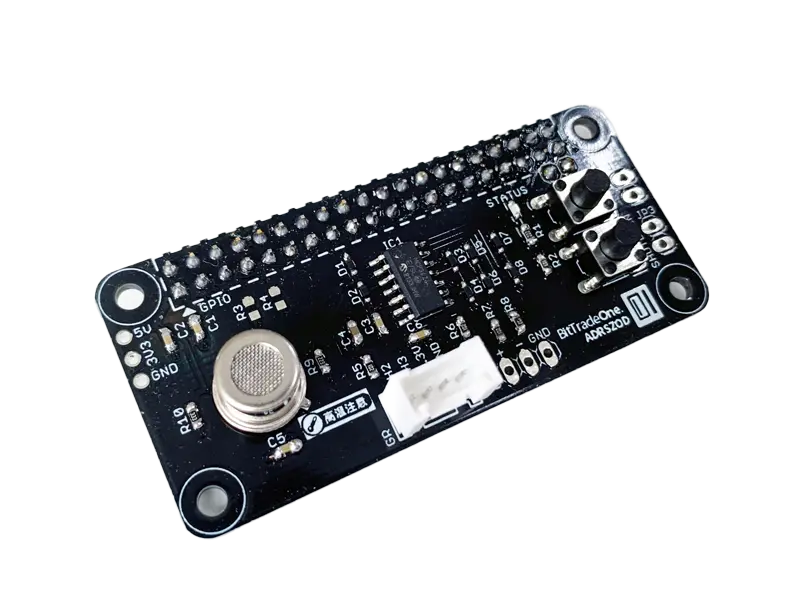
\includegraphics[keepaspectratio, scale=0.25]{figs/png/nioi_sensor.png}
		%		\caption{ADRSZOD:TP401A}
	\end{minipage}
\end{figure}

%\subsection{処理の概要}

\newpage

\subsection{cronによる時刻指定の処理}

cronの仕組みを使う(3つの時刻指定の処理を登録している)
\begin{enumerate}
	\item[(1)] 5分ごとに、リモートセンサの値を読み取る処理、rsensor.sh を起動する
	\item[(2)] 毎日23時56分になったら、その日1日分の測定データを退避する処理、daily.sh を起動する
	\item[(3)] 毎週日曜日の朝0時1分になったら、先週1週間の(先週の日曜日の0時0分から昨日の土曜日の23時55分まで5分間隔で測定した)測定データをまとめる処理、weekly.sh を起動する
\end{enumerate}

\begin{itembox}[l]{crontab -e}
	\begin{verbatim}
		MAILTO=""
		*/5 * * * * sh /home/mat/Documents/rsensor.sh
		56 23 * * * sh /home/mat/Documents/daily.sh
		1 0 * * Sun sh /home/mat/Documents/weekly.sh
	\end{verbatim}
\end{itembox}

ここで、MAILTO="" としているのは、「指定時刻にcronが処理を起動したよ」というメールを送信するためにsmtpを起動しようとして失敗し、指定の処理が起動されないという現象に対する対応である\footnote{postfixやsendmailなど、SMTPの何某かをインストールせよという説もあるが、特にメールの知らせが不要ならこのやり方が最も簡易な解決方法になる}

\begin{screen}
	\begin{verbatim}
		+---------------- minute (0 - 59)
		|  +------------- hour (0 - 23)
		|  |  +---------- day of month (1 - 31)
		|  |  |  +------- month (1 - 12)
		|  |  |  |  +---- day of week (0 - 6) (Sunday=0 or 7)
		|  |  |  |  |
		*  *  *  *  *  command to be executed
	\end{verbatim}
\end{screen}

%daily.shとweekly.shを、shではなくbashによって起動させているのは、それぞれのshellの中でのPythonの仮想環境への移行が、shでは移行できないという現象があったため、bashで運用することとしたもの

\newpage

\subsection{リモートセンサの処理をローカルマシンから起動する}

リモート(192.168.3.27)のRaspberry Pi Zero W に接続されている臭気センサの値を読みとるshell(sensor.sh)を、ローカル(192.168.3.21)のマシンRaspberry Pi からssh を使って起動するための shell(rsensor.sh)であり、cronによって5分ごとに起動される

この時sshから、リモートマシン(Pi Zero)のユーザ(今の環境ではmat)のパスワードを要求されるが、人手によるインタラクティブな入力操作を想定していないので、予めsshpassを導入しておいて、それによってパスワードを自動応答させる様にしている

sshでリモートのshellを実行した結果を受け取り、ローカルのw.txtに追記し蓄積していっている

\begin{itembox}[l]{/home/mat/Documents/rsensor.sh}
	\begin{verbatim}
#!/usr/bin/sh
### sudo apt install -y sshpass ###
dir='/home/mat/Documents'
addr='192.168.3.27'
usr='mat'
pass='mypassword'
sshpass -p ${pass} ssh ${usr}@${addr} \
  "bash ${dir}/sensor.sh" >> ${dir}/w.txt
	\end{verbatim}
\end{itembox}

w.txtの様子は、tail -f w.txt などとしてみると、5分ごとに起動されたshell(rsensor.sh)によって、測定結果が蓄積されていく様子がわかる(このファイルは、1日の終わりの処理で 2024-04-16.txt の様に、日付をつけたファイル名に変えて保存している)

\begin{itembox}[l]{w.txt -> 2024-04-16.txt}
	\begin{verbatim}
		2024-04-16, 00:35:04	ch1:1.0896
		2024-04-16, 00:40:04	ch1:1.09016
		2024-04-16, 00:45:04	ch1:1.09322
		.... ....
		2024-04-16, 23:45:04	ch1:0.9059
		2024-04-16, 23:50:04	ch1:0.99653
		2024-04-16, 23:55:04	ch1:0.98809
	\end{verbatim}
\end{itembox}

\subsection{日毎の処理}

毎日の23時55分に、その日の最後の測定が終わる事を前提として、cronには23時56分になったら次のshell(daily.sh)を起動する様にしている

このshellでは、現在時刻が23時55分を超えていることを確認した上で、次のことを行っている
\begin{itemize}
	\item 蓄積された1日分の測定データ w.txt を、bkup.txt という名前のファイルにコピーしている
	\item w.txt を、dataフォルダ以下に、「今日の日付.txt」 という名前に変更して保存している
	\item 空のファイル w.txt を次の日の測定データの蓄積場所のために用意している( touch)
	\item Pythonの仮想環境venv11に入って、daily.py を起動している(第1引数にdataフォルダ以下に保存した測定データファイルの名前=年月日を指定している)
	\item プログラムの実行を終えたら、Pythonの仮想環境venv11から抜けている
\end{itemize}

\begin{itembox}[l]{/home/mat/Documents/daily.sh}
	\begin{verbatim}
#!/usr/bin/sh
dir='/home/mat/Documents'
dates=$(date +%Y-%m-%d)
hour=$(date +%H)
minu=$(date +%M)
if [ ${hour} -ge 23 ]; then
  if [ ${minu} -gt 55 ]; then
    cp ${dir}/w.txt ${dir}/bkup.txt
    mv ${dir}/w.txt ${dir}/data/${dates}.txt
    touch ${dir}/w.txt
    . ${dir}/venv11/bin/activate
      python3 ${dir}/daily.py ${dates}
    deactivate
  fi
fi
	\end{verbatim}
\end{itembox}

%\newpage

\subsection{日毎処理のプログラム}

%\begin{itemize}
	myplot.py から、graph\_plot() 関数をimport している(この関数の詳細は後述)
	
	第1引数に指定があったら、そこで指定された日付のデータを元に、グラフを描画できる様にしている
	
	指定のデータファイルを開いて、最初の20文字までは、予めmatplotlibのdatesに対応した様式の日付文字列にしているので、それをUnixの日付けに変換している
	
	25文字目以降は、測定した電圧の値だが、改行文字が付いていたりするので、.strip()によってホワイトスペースを除去して、実数に変換している
	
	日付と電圧のリストを作って、それをgraph\_plot()関数に渡して作図させている
%\end{itemize}

\begin{itembox}[l]{/home/mat/Documents/daily.py}
	\begin{verbatim}
import sys
from datetime import datetime as dt
import matplotlib.dates as mdates
from myplot import graph_plot

dirstr = '/home/mat/Documents'
today = dt.now().strftime('%Y-%m-%d')
if len(sys.argv) > 1:
  today = sys.argv[1]

list0=[]
with open(dirstr + "/data/" + today + ".txt") as f:
  for line in f:
    datestr = line[:20].strip()
    datev = mdates.datestr2num(datestr)
    value = float(line[25:].strip())
    list0.append([datev, value])

title = 'Smel Level : ' + today
fig = graph_plot(list0, title)
#fig.savefig(dirstr + '/figs/' + today + '.png')
	\end{verbatim}
\end{itembox}

\newpage

このPythonのプログラムを実行した結果として、次の様な1日分のデータの変化をグラフ化したものが得られる%(これはfigsフォルダ以下に 「今日の日付.png」 という名称で保存している)

\begin{figure}[htbp]
	\begin{minipage}[b]{1.0\linewidth}
		\centering
		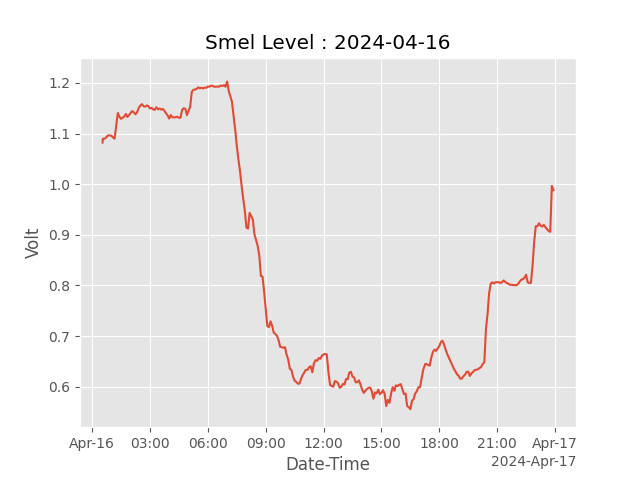
\includegraphics[keepaspectratio, scale=0.8]{figs/png/2024-04-16.png}
		\caption{daily.pyの出力(4月16日の0時から24時まで)}
	\end{minipage}
	%\hspace{1.0cm}
	%\begin{minipage}[b]{0.45\linewidth}
	%\centering
	%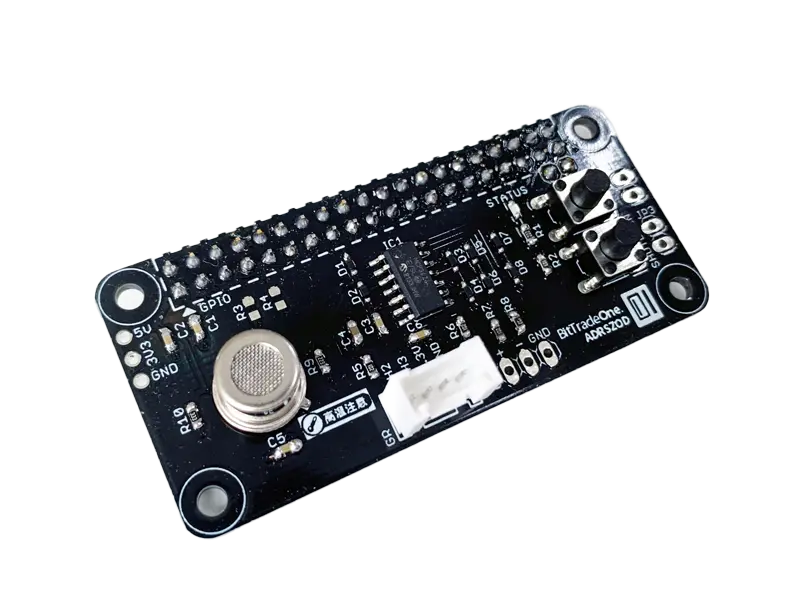
\includegraphics[keepaspectratio, scale=0.25]{figs/png/nioi_sensor.png}
	%\caption{ADRSZOD:TP401A}
	%\end{minipage}
\end{figure}

\subsection{グラフ描画のための関数}

daily.py と weekly.py で共通に呼び出しているgraph\_plot()関数を、以下の様に定義している

横軸に日付と時刻(データは5分毎)を置くため、少し工夫が必要になる

ポイントは、matplotlibが理解する日付の様式で書いたものを使うことさえできれば、matplotlibのdatesに、locatorとformatterを自動生成させ、それ以下の全ての面倒な処理を任せきることができる\footnote{\url{https://matplotlib.org/stable/api/dates_api.html}
	の記事が参考になる}点にある

\begin{itembox}[l]{/home/mat/Documents/myplot.py}
	\begin{verbatim}
		import numpy as np, pandas as pd
		from matplotlib import pyplot as plt, style, dates as mdates
		
		def graph_plot(list0, titlestr):
		  df = pd.DataFrame(list0, columns=["DateVal", "Value"])
		  matplotlib.style.use('ggplot')
		  fig, ax = plt.subplots()
		  x = df.loc[:,"DateVal"].values
		  y = df.loc[:,"Value"].values
		  locator = mdates.AutoDateLocator()
		  formatter = mdates.ConciseDateFormatter(locator)
		  ax.xaxis.set_major_locator(locator)
		  ax.xaxis.set_major_formatter(formatter)
		  ymin, ymax = y.min(), y.max()
		  step = (ymax - ymin) / 10.0
		  ymax = ((ymax // step) + 1) * step + step/2.0
		  ymin = (ymin // step) * step - step/2.0
		  ax.set_ylim([ymin, ymax])
		  ax.set_xlabel('Date-Time')
		  ax.set_ylabel('Volt')
		  ax.set_title(titlestr)
		  ax.plot(x,y)
		  plt.show()
		  return fig
	\end{verbatim}
\end{itembox}

%グラフの図を自動的に保存する様にしたいなら、最後の fig.savefig(...) のコメントを外して有効にする

\newpage

\subsection{週毎の処理}

この処理はcronによって、毎週日曜日の朝0時1分に起動される

このshell(weekly.sh)では、0時0分より後の時刻ならば仮想環境venv11に移って、Python のプログラム(weekly.py)を起動し、終わったら仮想環境鵜から抜けている

Pythonのプログラムは、第1引数に日付を受け取ることができる様にしている

\begin{itembox}[l]{/home/mat/Documents/weekly.sh}
	\begin{verbatim}
#!/usr/bin/sh
dir='/home/mat/Documents'
dates=$(date +%Y-%m-%d)
hour=$(date +%H)
minu=$(date +%M)
if [ ${hour} -ge 0 ]; then
  if [ ${minu} -gt 0 ]; then
    . ${dir}/venv11/bin/activate
      python3 ${dir}/weekly.py ${dates}
    deactivate
  fi
fi
	\end{verbatim}
\end{itembox}

\subsection{週毎処理のプログラム}

%\begin{itemize}
	myplot.pyからgraph\_plot()関数をimportしている
	
	第1引数で処理対象にする最終日付を受け取ることができる様にしている
	
	指定された処理対象の最終日付から、7日前の日付を求めて、7日間の日付のリストdatelistを作っている
	
	7日間の日付リストdatelistから1日ずつ取り出しては、そのファイル名のデータをdataフォルダから読み出し、日付の変換と電圧の実数への変換を行い、それらのデータのリストをlist0に追記していっている
	
	もし、指定した日付のデータファイルがなかった場合は、例外処理で受けて黙って次の日付のファイルのデータ取得に移る様にしている
	
	graph\_plot()関数にlist0を渡してグラフの作図をさせている
%\end{itemize}
\begin{spacing}{0.87}
\begin{itembox}[l]{/home/mat/Documents/weekly.py}
	\begin{verbatim}
from datetime import datetime as dt, timedelta
import sys, matplotlib.dates as mdates
from myplot import graph_plot

dirstr = '/home/mat/Documents'
s_format = '%Y-%m-%d'
today = dt.now()
if len(sys.argv) > 1:
  today = dt.strptime(sys.argv[1], s_format)
startstr = (today - timedelta(days=7)).strftime(s_format)

datelist = []
for i in range(7):
  day = today - timedelta(days=(7-i))
  datelist.append(day.strftime(s_format))

list0=[]
for fname in datelist:
  try:
    with open(dirstr + "/data/" + fname + ".txt") as f:
      for line in f:
        datestr = line[:20].strip()
        datev = mdates.datestr2num(datestr)
        value = float(line[25:].strip())
        list0.append([datev, value])
  except FileNotFoundError:
    continue

title = 'Smel Level : ' + startstr + ' (Weekly)'
fig = graph_plot(list0, title)
#fig.savefig(dirstr + '/figs/' + startstr + '.png')
	\end{verbatim}
\end{itembox}
\end{spacing}

%\newpage

以下は、週毎処理が出力する画像である。4月21日(日曜日)の0時1分にcronによって起動され実行されたものだが、フォルダdataの中には、測定を始めた4月16日(火曜日)から、4月20日(土曜日)までの5日分のファイルがあるだけである。本来なら1週間前の日曜日(4月14日)のデータから週毎処理の対象となるところだが、プログラムの中ではFileNotFoundErrorの例外を捕捉して、とにかくcontinueによって処理を継続させているため、何事もなかったかの様に、データファイルの所在する火曜日以降がグラフに作図されている

また、日毎処理のプログラムdaily.pyと全く同じグラフ作図の関数(myplot.pyの中のgraph\_plot()関数)を使っているのだが、横軸の設定がmatplotlibのdates(mdatesとしてプログラム中では使っている)によって、自動的に調整されているのが分かる(便利)

\begin{figure}[htbp]
	\begin{minipage}[b]{1.0\linewidth}
		\centering
		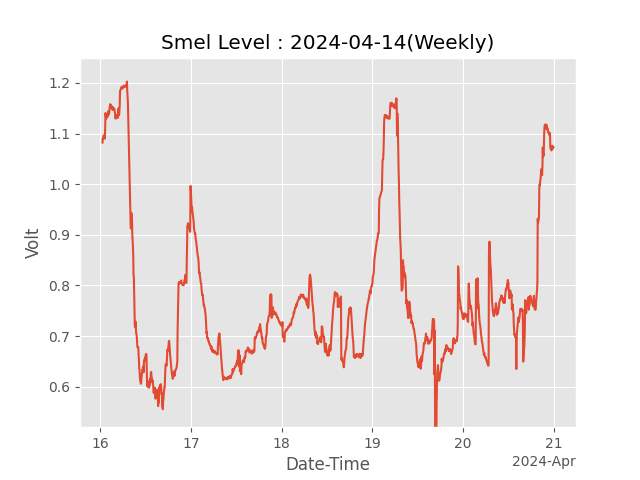
\includegraphics[keepaspectratio, scale=0.8]{figs/png/Weekly_2024-04-14.png}
		\caption{weekly.pyの出力}
	\end{minipage}
	%\hspace{1.0cm}
	%\begin{minipage}[b]{0.45\linewidth}
	%\centering
	%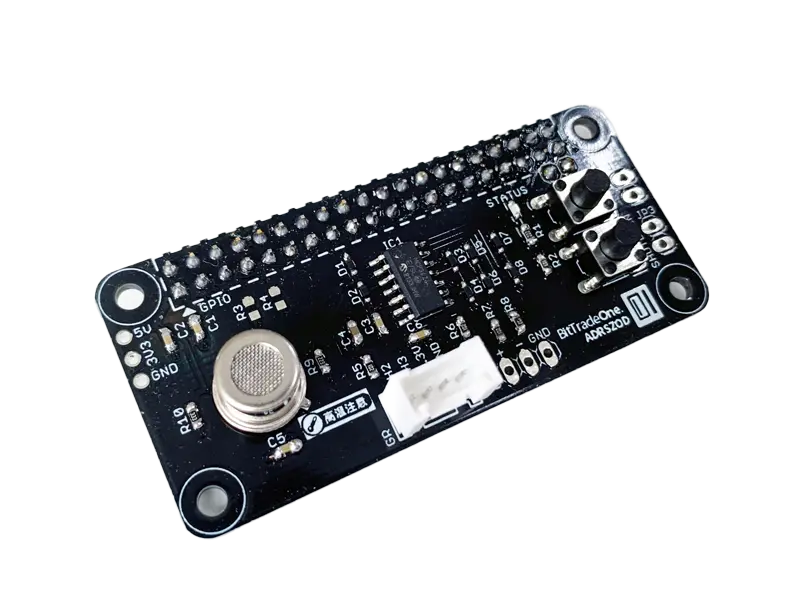
\includegraphics[keepaspectratio, scale=0.25]{figs/png/nioi_sensor.png}
	%\caption{ADRSZOD:TP401A}
	%\end{minipage}
\end{figure}

%\newpage

\subsection{測定データのグラフを実時間で描画する}

%\begin{itemize}
	RTPlotクラスは、実時間によるグラフ描画に必要な関数類をまとめたもの
	
	ポイントとなるのは、 plt.show() を使わず、plt.pause(1.0)を使うこと、tail -f をプログラム上で実現することの2点
	
	self.xとself.yのリストに順にデータを追記していき、新たなデータがw.txtに追加されたタイミングでplt.pause(1.0)としている(引数の値を0.1や0.01にするとRaspberry Piでは全て描画しきれないので注意)
	
	tail\_f()関数は、コマンド tail -f w.txt をPythonのプログラムで実現したもの(指定したファイルの最終行が追記されるまでcontinueで待っている)である
%\end{itemize}

\begin{spacing}{0.87}
\begin{breakbox}%[l]{/home/mat/Documents/rtplot.py}
	\begin{verbatim}
import sys, time, numpy as np
from datetime import datetime as dt, timedelta
from matplotlib import pyplot as plt, dates as mdates, style

class RTPlot:
  def dt2str(self, dat, sformat):
    return dat.strftime(sformat)

  def str2dt(self, str, sformat):
    return dt.strptime(str, sformat)

  def dateproc(self, datestr):
    #s_format = '%Y-%m-%d, %H:%M:%S'
    s_format0 = '%Y-%m-%d, 00:00:00'
    self.today = dt.now()
    self.todaystr = self.dt2str(self.today, s_format0)
    if datestr != 'w' and datestr != self.todaystr[:10]:
      self.today = self.str2dt(datestr, '%Y-%m-%d')
      self.todaystr = self.dt2str(self.today, s_format0)
    self.tomorrow = self.today + timedelta(days=1)
    self.tomorstr = self.dt2str(self.tomorrow, s_format0)

  def readdata(self, fname):
    try:
      with open(fname, 'r') as f:
        for line in f:
          self.chop(line)
    except FileNotFoundError:
      print(f'File{fname} not found')

  def __init__(self, datestr, fpath):
    self.fname = fpath + datestr + '.txt' 
    self.x = []
    self.y = []
    self.ims = []
    self.dateproc(datestr)
    self.readdata(self.fname)
    matplotlib.style.use('ggplot')
    self.fig, self.ax = plt.subplots()
    locator = mdates.AutoDateLocator()
    formatter = mdates.ConciseDateFormatter(locator)
    self.ax.xaxis.set_major_locator(locator)
    self.ax.xaxis.set_major_formatter(formatter)
    xmin = mdates.datestr2num(self.todaystr)
    xmax = mdates.datestr2num(self.tomorstr) 
    self.ax.set_xlim([xmin, xmax])
    self.yrange()
    self.ax.set_xlabel('Date-Time')
    self.ax.set_ylabel('Volt')
    self.update()

  def chop(self, line):
    datestr = line[:20].strip()
    datev = mdates.datestr2num(datestr)
    value = float(line[25:].strip())
    self.x.append(datev)
    self.y.append(value)

  def tail_f(self):
    try:
      with open(self.fname, 'r') as f:
        f.seek(0, 2)
        enter = dt.now()
        while True:
          line = f.readline()
          if not line:
            time.sleep(1)
            if dt.now()-enter < timedelta(minutes=6):
              continue
            return
          return line.strip()
    except FileNotFoundError:
      print(f'File{self.fname} not found')
    return

  def statvalue(self):
    self.ymax = np.array(self.y).max()
    self.ymin = np.array(self.y).min()
    self.mean = np.array(self.y).mean()
    str1 = f"Max={self.ymax:.2f}, "
    str2 = f"Min={self.ymin:.2f}, "
    str3 = f"Mean={self.mean:.2f}"
    self.ax.set_title("Smel Level : " + str1 + str2 + str3)

  def yrange(self):
    self.statvalue()
    step = (self.ymax - self.ymin)/10.0
    v = 0
    while self.ymax > v:
      v += step
    ymax = v + step/2.0
    while self.ymin < v:
      v -= step
    ymin = v - step/2.0
    self.ax.set_ylim([ymin, ymax])

  def update(self):
    self.yrange()
    if len(self.ims) > 0:
      im = self.ims.pop()
      im.remove()
    im, = self.ax.plot(self.x, self.y, color='red')
    self.ims.append(im)

if __name__ == "__main__":
  dirstr = '/home/mat/Documents'
  datestr = 'w'
  fpath = dirstr + '/'
  if len(sys.argv) > 1:
    datestr = sys.argv[1]
    fpath = dirstr + '/data/'
  rtp = RTPlot(datestr, fpath)
  while dt.now() < rtp.tomorrow:
    plt.pause(1)
    line = rtp.tail_f()
    if line is not None:
      print("[info.log]", line)
      rtp.chop(line)
      rtp.update()
  rtp.fig.savefig(dirstr + '/figs/R_' + rtp.todaystr[:10] + '.png')
	\end{verbatim}
\end{breakbox}
\end{spacing}

\newpage

tail\_f()関数の中では、6分を超えてcontinueを繰り返している場合にNoneを返す事にしている(6分待てば、その間には必ず5分間隔のイベントは入ってくると思う)ので、mainの中の繰り返し処理whileの中でその事を(PEP8が可読性の観点から推奨している書き方) is not None によって判定している

実時間処理の画面は次の様になる.

このプログラム rtplot.py が終了時に保存する画像は、実は日毎処理のプログラム daily.py が出力するものとほぼ同じ傾向を示しているはずだ。ただ rtplot.py の方は、新たな点をプロットするたびにy軸の最大値と最小値を更新しているため、日毎の処理では作図の範囲外に出るデータも示せているし、また具体的な最大値、最小値、平均値の値もその都度更新して表示している

\begin{figure}[htbp]
	\begin{minipage}[b]{1.0\linewidth}
		\centering
		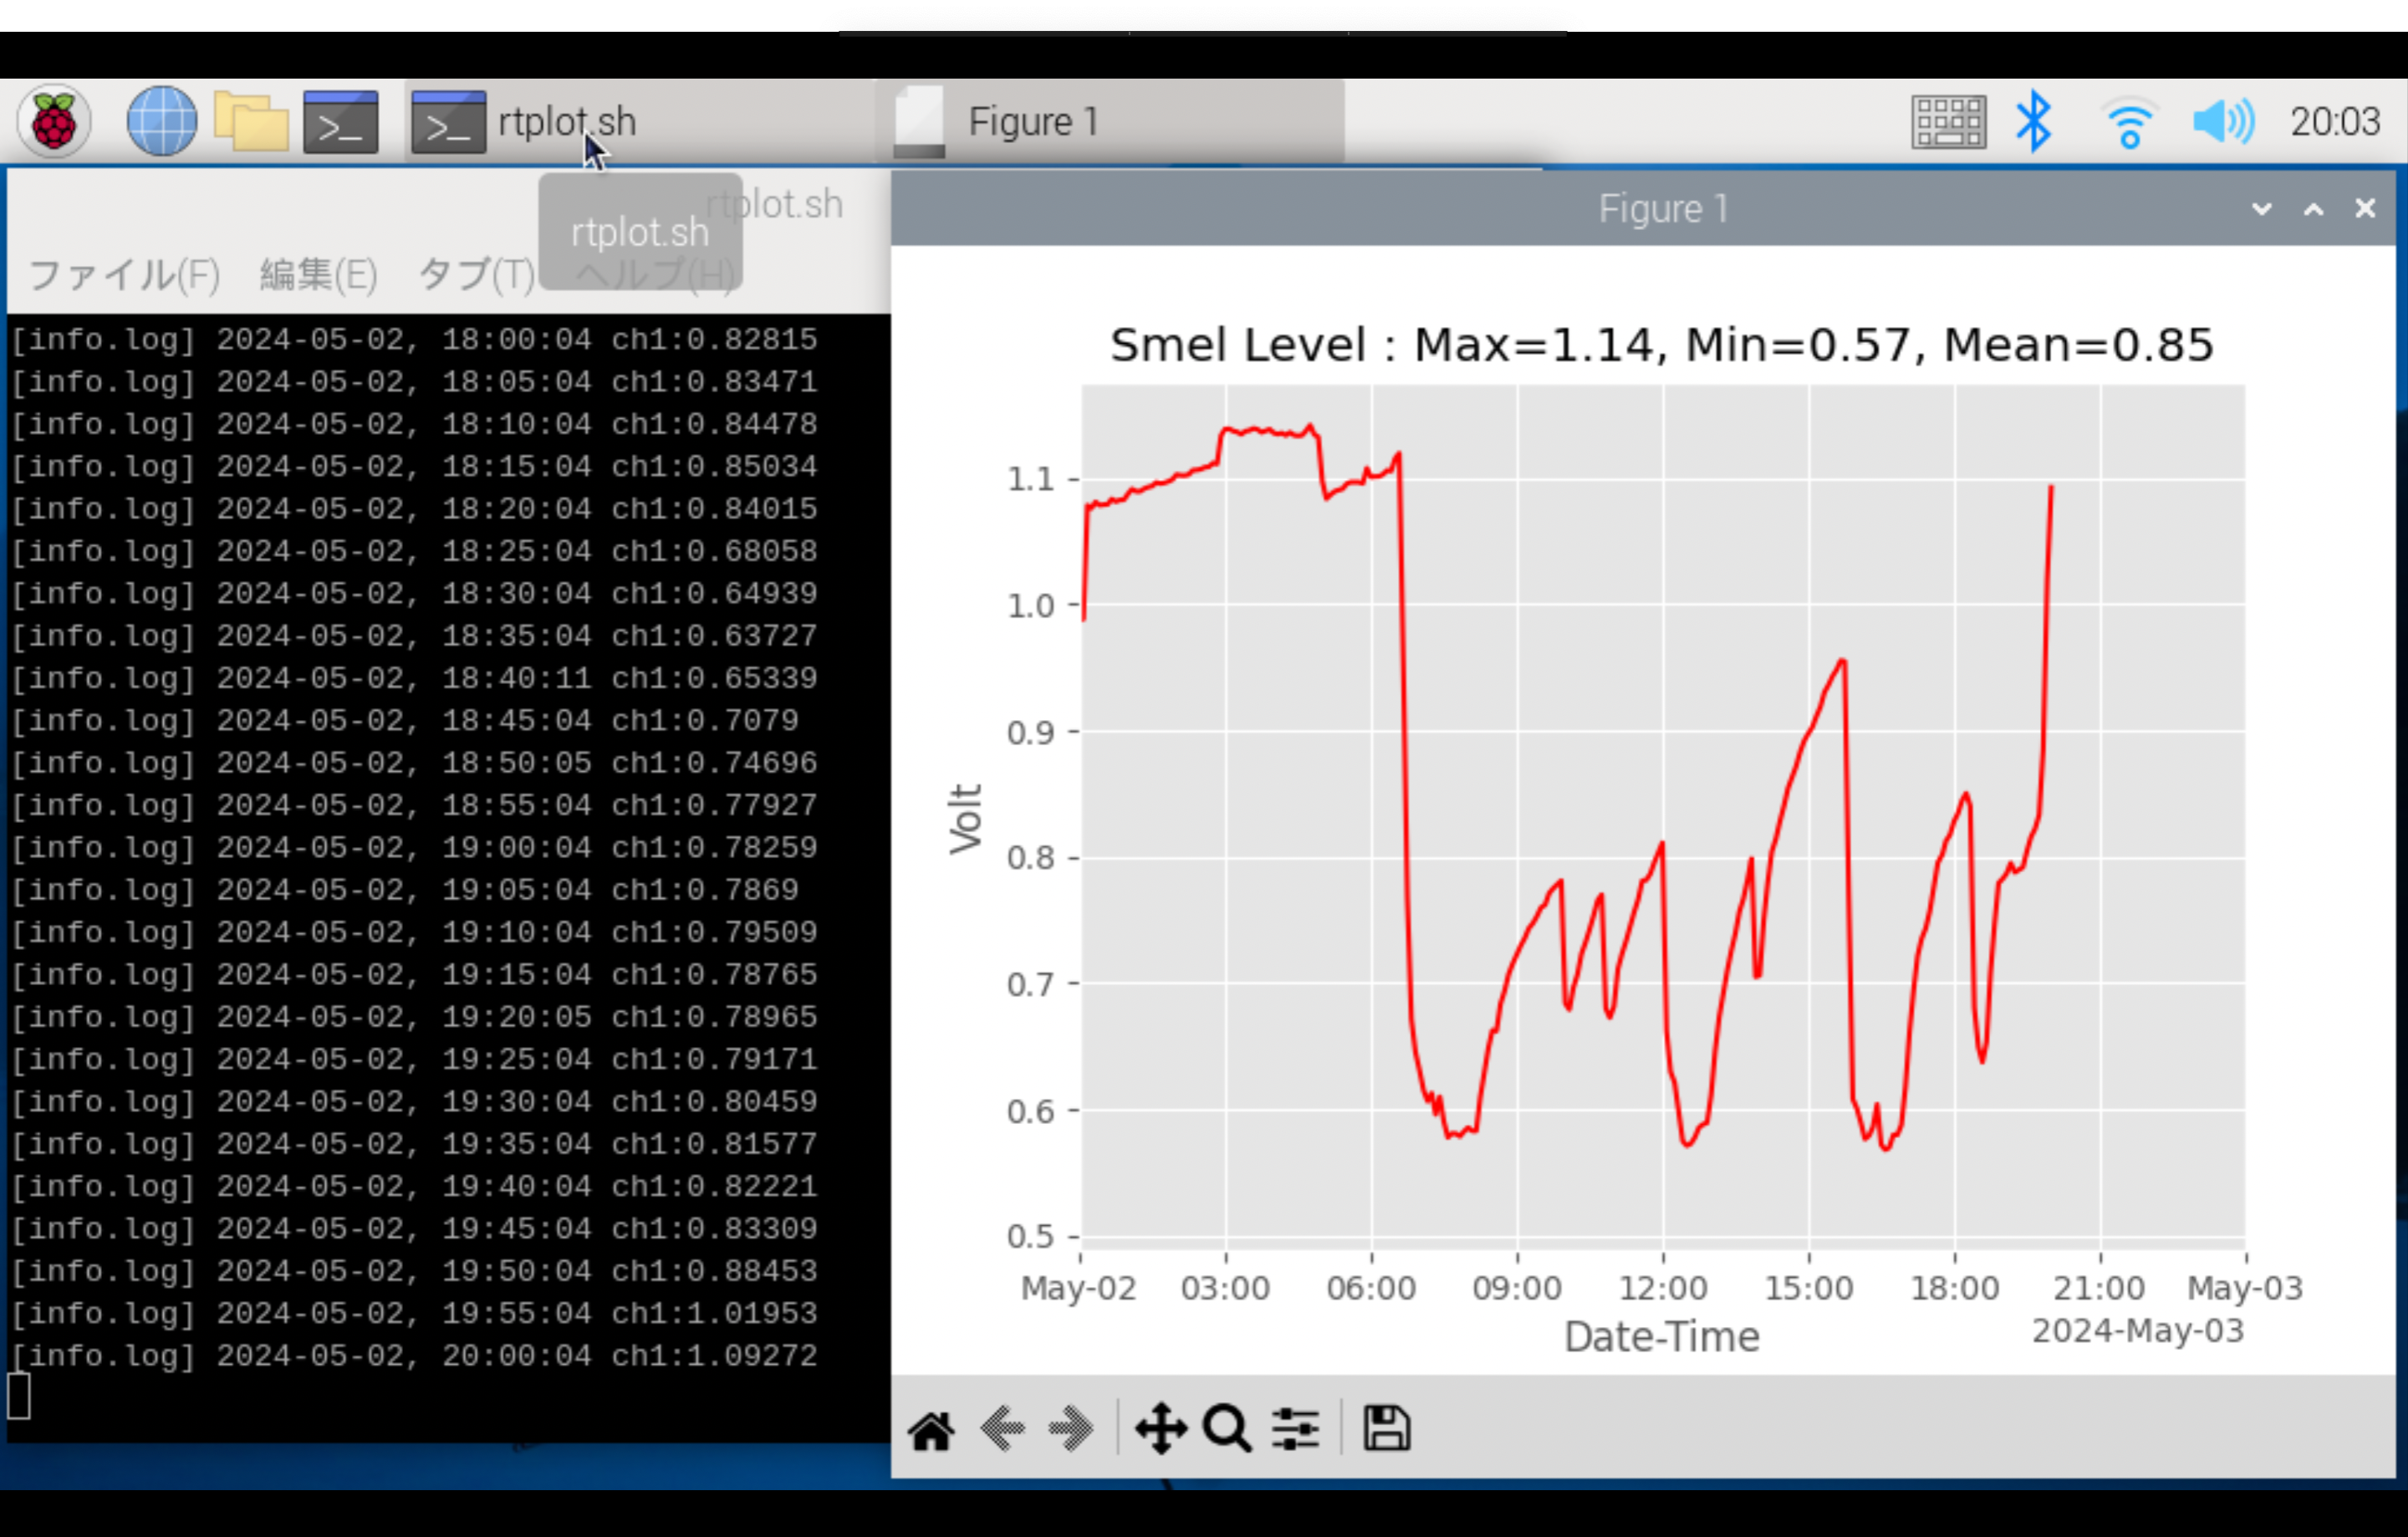
\includegraphics[keepaspectratio, scale=0.26]{figs/png/screen2.png}
		\caption{実時間出力(途中経過:5月2日の20時過ぎ)}
	\end{minipage}
	%\hspace{1.0cm}
	%\begin{minipage}[b]{0.45\linewidth}
	%\centering
	%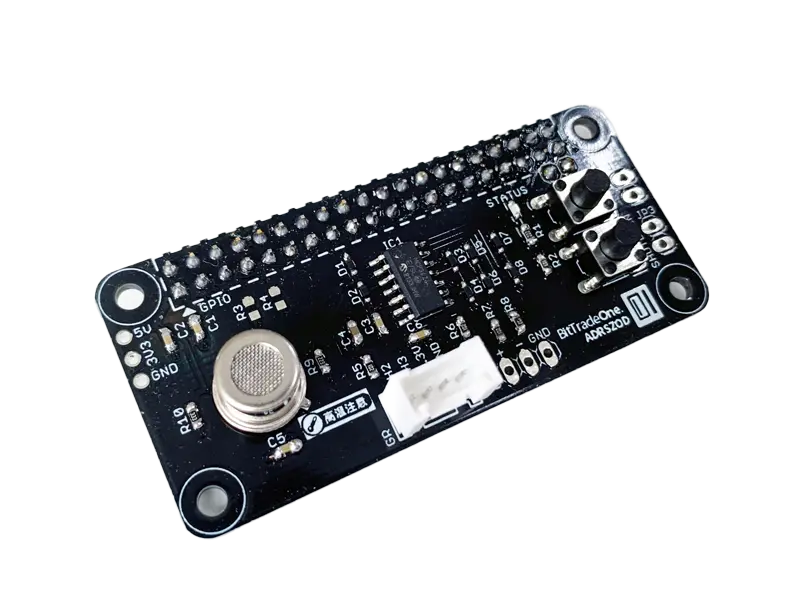
\includegraphics[keepaspectratio, scale=0.25]{figs/png/nioi_sensor.png}
	%\caption{ADRSZOD:TP401A}
	%\end{minipage}
\end{figure}

この実時間プロットのプログラムを起動するshellを、実行可能属性を持たせてデスクトップに置いている(マウスのクリックで起動できる)

\begin{itembox}[l]{/home/mat/Desktop/rtplot.sh}
	\begin{verbatim}
		#!/usr/bin/sh
		dir='/home/mat/Documents'
		cd ${dir}
		. ${dir}/venv11/bin/activate
		  python3 ${dir}/rtplot.py
		deactivate
	\end{verbatim}
\end{itembox}

日付の文字列を第1引数に指定して、コマンドラインから直接実行すると、
\begin{verbatim}
	cd /home/mat/Documents
	source venv11/bin/activate
	  python3 rtplot.py 2024-05-10
	deactivate
\end{verbatim}
その日付けのデータに基づく実時間グラフをfigsフォルダの中に生成する

%このshellは、/usr/bin/sh で動かそうとすると「はて?source って何のこと?」などと言ってくるので、/usr/bin/bash で動かす様にする

%\newpage

\chapter{リモートにデータを保持する}

\begin{table}[h]
	\centering
	\caption{ここで使用するshellとプログラム}
	\label{tab:local}
	\begin{tabular}{llp{8.5cm}}
		\hline
		リモート & sensor.sh{*} & 日付文字列とセンサーの読み取り値を並べて出力するshell \\
		リモート & adrsz0D.py{*} & センサーを読むクラスの定義 \\
		リモート & procmain.py{*} & センサーのインスタンス生成とセンサーの読取り \\
		リモート & proc.sh & cron により5分間隔で起動される. sensor.sh を起動して w.txt に計測データを追記蓄積する \\
		リモート & procdaily.sh & cron により毎日23時58分に起動される. 1日分の蓄積データ w.txt をdata/フォルダへ退避させる \\
		ローカル & lackdata.py & data/フォルダ内に、本日の日付までで保存されていないデータがあったら、その日付の一覧を標準出力へ出力する \\
		ローカル & lack.sh & lackdata.py が出力する日付をパイプを介した標準入力で受け、その日付のデータが、ローカルの w.txt、リモートの w.txt、リモートのdata/フォルダ内、ローカルのdata/フォルダ内にないか、すべて探し出してマージし、その日付のファイルとしてローカルのdata/フォルダに保存する  \\ \hline
	\end{tabular}
\end{table}

\section{リモートマシンの処理}

リモートとローカルの両方を動かし続けるのが難しい場合に、
普段はリモートだけにデータを集めておいて、
時々ローカルにリモートのデータを取り込み、
それをグラフ化するなどの処理を行う方法をとる運用も考えられる

%\subsection{リモートマシンでの処理}

リモートのコンピュータ内でデータを集める仕組みは、
ほぼローカルコンピュータでの処理と同様にして実施する

\begin{itembox}[l]{/home/mat/Documents/proc.sh}
	\begin{verbatim}
#!/usr/bin/sh
dir='/home/mat/Documents'
bash ${dir}/sensor.sh >> ${dir}/w.txt
	\end{verbatim}
\end{itembox}

リモートにも、(ローカルと同様のディレクトリ構成で)/home/mat/Documents/data フォルダを用意しておく

\begin{itembox}[l]{/home/mat/Documents/procdaily.sh}
	\begin{verbatim}
#!/usr/bin/sh
dir='/home/mat/Documents'
dates=$(date +%Y-%m-%d)
hour=$(date +%H)
minu=$(date +%M)
if [ ${hour} -ge 23 ]; then
  if [ ${minu} -gt 57 ]; then
    cp ${dir}/w.txt ${dir}/bkup.txt
    mv ${dir}/w.txt ${dir}/data/${dates}.txt
    touch ${dir}/w.txt
  fi
fi
	\end{verbatim}
\end{itembox}

crontab では、5分ごとの処理を(ローカルマシンの処理時刻とずらすため)、2,7,12,17,... の5分おきに実行される様にした

\begin{itembox}[l]{crontab -e}
\begin{verbatim}
MAILTO=""
# m h  dom mon dow   command
2-57/5 * * * * sh /home/mat/Documents/proc.sh
58 23 * * * sh /home/mat/Documents/procdaily.sh
\end{verbatim}	
\end{itembox}

\newpage

\section{ローカルマシンの処理}

Pythonのプログラムで、ローカルマシン内に欠けている日付のデータファイルを調べる

\begin{itembox}[l]{/home/mat/Documents/lackdata.py}
	\begin{verbatim}
from datetime import datetime as dt, timedelta
import glob

s_format = '%Y-%m-%d'
todaystr = (dt.now() + timedelta(days=0)).strftime(s_format)
today = dt.strptime(todaystr, s_format)

dirstr = '/home/mat/Documents'
wlist = glob.glob(dirstr + '/data/*.txt')
dlist = []
for w in wlist:
  dlist.append(dt.strptime(w[len(dirstr)+6:-4], s_format))
dlist.sort(reverse=True)	# descending order

ten_days = 10
lacklist = []
for d in range(ten_days):
  day = today - timedelta(days=d)
  if day in dlist:
    continue
  else:
    lacklist.append(day)

for fname in lacklist:
  print(fname.strftime(s_format))
	\end{verbatim}
\end{itembox}

このプログラムを実行した段階で、
ローカルに無いファイル(名前の日付の部分)が分かったので、
ローカルとリモートのマシンからその日付のデータを集めて整理する
%(リモートマシン上のデータファイルで、ローカルマシンに取り込みが済んだものは、手動で削除する運用とする)
\begin{itembox}[l]{/home/mat/Documents/lack.sh}
	\begin{verbatim}
#!/usr/bin/sh
TODAY=$(date +%Y-%m-%d)
PASS='mypassword'
USR='mat'
ADDR='192.168.3.27'
DIR='/home/mat/Documents'
cp ${DIR}/w.txt ${DIR}/bkup.txt
. ${DIR}/venv11/bin/activate
  python3 ${DIR}/lackdata.py | \
while read LINE; do (
  grep ^${LINE} ${DIR}/bkup.txt > ${DIR}/${LINE}.wrk
  sshpass -p ${PASS} ssh -n ${USR}@${ADDR} \
    "grep ^${LINE} ${DIR}/w.txt" >> ${DIR}/${LINE}.wrk
  CMD=test\ -e\ ${DIR}/data/${LINE}.txt
  RC=$(sshpass -p ${PASS} ssh -n ${USR}@${ADDR} ${CMD};echo $?)
  if [ ${RC} -eq 0 ]; then
    sshpass -p ${PASS} ssh -n ${USR}@${ADDR} \
      "grep ^${LINE} ${DIR}/data/${LINE}.txt" >> ${DIR}/${LINE}.wrk
  fi
  sort ${DIR}/${LINE}.wrk | uniq - > ${DIR}/${LINE}.wrk2
  rm ${DIR}/${LINE}.wrk
  if [ -s ${DIR}/${LINE}.wrk2 ]; then
    match=$(echo ${LINE} | awk "/^${TODAY}/")
    if [ -n "${match}" ]; then
      cp ${DIR}/${LINE}.wrk2 ${DIR}/w.txt
    else
      cp ${DIR}/${LINE}.wrk2 ${DIR}/data/${LINE}.txt
    fi
  fi
  rm ${DIR}/${LINE}.wrk2
) < /dev/null; done
deactivate
	\end{verbatim}
\end{itembox}

%\newpage

\chapter{クラウド上にデータを保持する}

\begin{table}[h]
	\centering
	\caption{ここで使用するshellとプログラム}
	\label{tab:local}
	\begin{tabular}{p{1.3cm}lp{8.5cm}}
		\hline
		リモート & sensor.sh{*} & 日付文字列とセンサーの読み取り値を並べて出力するshell \\
		リモート & adrsz0D.py{*} & センサーを読むクラスの定義 \\
		リモート & procmain.py{*} & センサーのインスタンス生成とセンサーの読取り \\
		リモート & proc.sh{*} & cron により5分間隔で起動される. sensor.sh を起動して w.txt に計測データを追記蓄積する \\
		リモート & procdaily.sh & cron により毎日23時58分に起動される. 1日分の蓄積データ w.txt をdata/フォルダへ退避させる. upcloud.py を起動して本日分の計測データをクラウドにアップロードし、最後に昨日分の計測データを削除する(更新) \\
		リモート & upcloud.py & クラウドに指定日付のデータをアップロードする.  \\
		ローカル & mycloud.py & 指定した日付のデータをクラウドから読んで標準出力に出力する. -w のスイッチを付けて起動した場合、指定日付から1週間前までのデータをクラウドから読んで標準出力へ出力する.   \\
		ローカル & daily.py & 標準入力から受け取った計測データをもとに、1日の値の変化をグラフにする(更新) \\
		ローカル & weekly.py & 標準入力から受け取った計測データをもとに、1週間の値の変化をグラフにする(更新) \\
		ローカル & dayplot.sh & mycloud.py から daily.py へパイプで繋いでいる \\
		ローカル & weekplot.sh & mycloud.py から weekly.py へパイプで繋いでいる \\
		ローカル & myplot.py{*} & グラフ作図関数. daily.pyとweekly.py から呼び出される \\
		両方 & gcloud.py & GCSWapperクラス(upload0.pyとmycloud.pyで継承する) \\ \hline
	\end{tabular}
\end{table}

\section{リモートマシンの処理}

センサのデータを w.txt に蓄積していく処理は、これまでのものと同じ

\begin{itembox}[l]{/home/mat/Documents/proc.sh}
	\begin{verbatim}
		#!/usr/bin/sh
		dir='/home/mat/Documents'
		bash ${dir}/sensor.sh >> ${dir}/w.txt
	\end{verbatim}
\end{itembox}

procdaily.sh を次の様にする

\begin{enumerate}
\item[(1)] 1日分のデータ w.txt を bkup.txt に退避して
\item[(2)] それを /home/mat/Documents/data/フォルダ内に、日付をファイル名として保存し
\item[(3)] そのファイルをクラウドへアップロードする
\item[(4)] その日の終わりに、昨日分のデータを削除する
\end{enumerate}

こうして、リモートマシン内には当日集めているデータ w.txt、バックアップの1日分のデータ bkup.txt、ファイル名に日付を付けた1日分のデータの、3つしか保持していない(日々のデータはクラウド上にある)

\begin{itembox}[l]{/home/mat/Documents/procdaily.sh}
	\begin{verbatim}
		#!/usr/bin/sh
		dir='/home/mat/Documents'
		dates=$(date +%Y-%m-%d)
		hour=$(date +%H)
		minu=$(date +%M)
		if [ ${hour} -ge 23 ]; then
		  if [ ${minu} -gt 57 ]; then
		    cp ${dir}/w.txt ${dir}/bkup.txt
		    mv ${dir}/w.txt ${dir}/data/${dates}.txt
		    touch ${dir}/w.txt
		    python3 ${dir}/upcloud.py ${dates}
		    yesterday=$(date --date "${dates} 1 days ago" +%Y-%m-%d)
		    rm ${dir}/data/${yesterday}.txt
		  fi
		fi
	\end{verbatim}
\end{itembox}

crontab では、proc.sh を 2,7,12,17,... の5分おきに実行する様にし、procdaily.sh は23時58分に実行する様にしている(proc.shがその日の最後に実行されるのは、23時57分だから)

\begin{itembox}[l]{crontab -e}
	\begin{verbatim}
		MAILTO=""
		# m h  dom mon dow   command
		2-57/5 * * * * sh /home/mat/Documents/proc.sh
		58 23 * * * sh /home/mat/Documents/procdaily.sh
	\end{verbatim}	
\end{itembox}

クラウドへ指定のファイルをアップロードする処理 upcloud.py は、ラッパークラスGCSWrapperを継承して、必要なメソッドを呼び出しているだけ(クラウド上にもdata/フォルダを用意して、そこに日付をファイル名とするファイルをアップロードしている)

\begin{itembox}[l]{/home/mat/Documents/upcloud.py}
	\begin{verbatim}
		from datetime import datetime as dt
		import sys
		from gcloud import GCSWrapper
		
		class cloud(GCSWrapper):
		   def __init__(self, proj_name, bkt_name):
		      super().__init__(proj_name, bkt_name)
		
		if __name__ == '__main__':
		   project_id = "myprojectid"
		   bucket_name = "mybucketname"
		   CL = cloud(project_id, bucket_name)
		   dirstr = '/home/mat/Documents'
		   path = dirstr + '/data/'
		   datestr = dt.now().strftime('%Y-%m-%d')
		   if len(sys.argv) > 1:
		     datestr = sys.argv[1]
		   CL.upload_file(path+datestr+'.txt', 'data/'+datestr+'.txt')		
	\end{verbatim}	
\end{itembox}

\newpage

\section{ローカルマシンの処理}

測定データが、日付ごとに名前をつけてクラウド上に保存されているので、ローカルではクラウドからデータを読んできて、日毎のグラフ、あるいは週毎のグラフを適時作図する処理とする

クラウドからファイルをダウンロードしてローカルに保存後、そのファイルを読み込んで処理するのではなく、標準入出力のパイプによる受け渡しの方法をとる方がエレガントだと思う(ローカルに保存されるファイルはない)
\subsection{日毎のグラフの作図}

\begin{enumerate}
\item[(1)] mycloud.py でクラウドから指定した日付のデータを読んできて、それを標準出力へ出力する
\item[(2)] mycloud.py の標準出力を、パイプを通して daily.py の標準入力で受け取り、グラフの作図を行う
\end{enumerate}

\begin{itembox}[l]{/home/mat/Documents/dayplot.sh}
	\begin{verbatim}
#!/usr/bin/sh
dir='/home/mat/Documents'
if [ $# -eq 1 ]; then
dates=$1
. ${dir}/venv11/bin/activate
   python3 ${dir}/mycloud.py ${dates} | python3 ${dir}/daily.py
deactivate
fi
	\end{verbatim}
\end{itembox}

次の様に動作させる(日付を第1引数に指定する)

\begin{screen}
\begin{verbatim}
	(venv11) mat@raspi:~/Documents $ sh ./dayplot.sh 2024-05-18
\end{verbatim}
\end{screen}

mycloud.py と daily.py は次の通り(同じ場所に myplot.py と gcloud.py を置いておく必要がある)

\begin{spacing}{0.87}
\begin{itembox}[l]{/home/mat/Documents/mycloud.py}
	\begin{verbatim}
from datetime import datetime as dt, timedelta
import sys, pandas as pd
from gcloud import GCSWrapper

class cloud(GCSWrapper):
   def __init__(self, proj_name, bkt_name):
      super().__init__(proj_name, bkt_name)

   def download_as_string(self, gcs_path):
      blob = self._bucket.blob(gcs_path)
      text = blob.download_as_string().decode()
      return text

if __name__ == '__main__':
   project_id = "myprojectid"
   bucket_name = "mybucketname"
   CL = cloud(project_id, bucket_name)
   #CL.show_file_names()
   dirstr = '/home/mat/Documents'
   path = dirstr + '/data/'
   s_format = '%Y-%m-%d'
   datestr = dt.now().strftime(s_format)
   if len(sys.argv) == 3 and sys.argv[1]=='-w':
      today = dt.strptime(sys.argv[2], s_format)
      datestr = (today - timedelta(days=7)).strftime(s_format)
      text = ""
      for i in range(7):
         day = today - timedelta(days=(7-i))
         datestr = day.strftime(s_format)
         try:
            temp = CL.download_as_string('data/'+datestr+'.txt')
         except FileNotFoundError:
            continue
         text += temp   
   else:
      datestr = sys.argv[1]
      text = CL.download_as_string('data/'+datestr+'.txt')
      for dstr in text.split('\n'):
         if len(dstr)>0:
            print(dstr[:20], '\t', dstr[25:].strip())
   \end{verbatim}
\end{itembox}
   \end{spacing}

\begin{spacing}{0.87}
	\begin{itembox}[l]{/home/mat/Documents/daily.py}
		\begin{verbatim}
			from datetime import datetime as dt
			import sys, matplotlib.dates as mdates
			from myplot import graph_plot
			
			dirstr = '/home/mat/Documents'
			today = dt.now().strftime('%Y-%m-%d')
			argv = len(sys.argv)
			if argv==2:
			   today = sys.argv[1]
			
			list0=[]
			if argv==2:
			   with open(dirstr + "/data/" + today + ".txt") as f:
			   for line in f:
			      datestr = line[:20].strip()
			      datev = mdates.datestr2num(datestr)
			      value = float(line[25:].strip())
			      list0.append([datev, value])
			else:
			   while True:
			      try:
			         line = input()
			         for i, l in enumerate(line.split('\t')):
			            temp = l.strip()
			            if len(temp)>0:
			               if i==0:
			                  today = temp[:10]
			                  datev = mdates.datestr2num(temp)
			               else:
			                  value = float(temp)
			            list0.append([datev, value])
			      except EOFError:
			         break

			title = 'Smel Level : ' + today
			fig = graph_plot(list0, title)
			#fig.savefig(dirstr + '/figs/' + today + '.png')
  	 	\end{verbatim}
	\end{itembox}
\end{spacing}

\subsection{1週間のグラフの作図}

\begin{enumerate}
	\item[(1)] mycloud.py でクラウドから、指定した日付からさかのぼって1週間分のデータを読んできて、それを標準出力へ出力する
	\item[(2)] mycloud.py の標準出力を、パイプを通して weekly.py の標準入力で受け取り、グラフの作図を行う
\end{enumerate}

\begin{itembox}[l]{/home/mat/Documents/weekplot.sh}
	\begin{verbatim}
#!/usr/bin/sh
dir='/home/mat/Documents'
if [ $# -eq 1 ]; then
dates=$1
. ${dir}/venv11/bin/activate
   python3 ${dir}/mycloud.py -w ${dates} | python3 ${dir}/weekly.py
deactivate
fi
	\end{verbatim}
\end{itembox}

mycloud.py では、-w のスイッチを指定することによって、1週間分のファイルをクラウドから読み込むことを指示している(ソースプログラムは日毎の処理で使ったものと同じ)

次の様に動作させる(1週間の最後の日付を第1引数に指定する)

\begin{screen}
	\begin{verbatim}
		(venv11) mat@raspi:~/Documents $ sh ./weekplot.sh 2024-05-18
	\end{verbatim}
\end{screen}

weekly.py は次の通り(日毎の処理と同様に、同じ場所に myplot.py と gcloud.py を置いておく必要がある)

\begin{spacing}{0.8}
	\begin{itembox}[l]{/home/mat/Documents/weekly.py}
		\begin{verbatim}
			import sys, matplotlib.dates as mdates
			from datetime import datetime as dt, timedelta
			from myplot import graph_plot
			
			dirstr = '/home/mat/Documents'
			today = dt.now()
			if len(sys.argv) > 1:
			   today = dt.strptime(sys.argv[1], '%Y-%m-%d')
			startstr = (today - timedelta(days=7)).strftime('%Y-%m-%d')
			datelist, list0 = [], []
			for i in range(7):
			   day = today - timedelta(days=(7-i))
			   datelist.append(day.strftime('%Y-%m-%d'))
			if sys.argv==2:
			   for fname in datelist:
			      try:
			         with open(dirstr + "/data/" + fname + ".txt") as f:
			            for line in f:
			               datestr = line[:20].strip()
			               datev = mdates.datestr2num(datestr)
			               value = float(line[25:].strip())
			               list0.append([datev, value])
			      except FileNotFoundError:
			         continue
			else:
			   while True:
			      try:
			         line = input()
			         for i, l in enumerate(line.split('\t')):
			            temp = l.strip()
			            if len(temp)>0:
			               if i==0:
			                  startstr = temp[:10]
			                  datev = mdates.datestr2num(temp)
			               else:
			                  value = float(temp)
			            list0.append([datev, value])
			      except EOFError:
			         break

			title = 'Smel Level : ' + startstr + ' (Weekly)'			
			fig = graph_plot(list0, title)
			#fig.savefig(dirstr + '/figs/' + startstr + '.png')
  	 	\end{verbatim}
\end{itembox}
\end{spacing}

\chapter{補遺}

\section{shell を記述する上での注意点}

\begin{itemize}
	\item 次の部分で、\$\{TODAY\}と\$\{match\}はダブルクオートで囲む必要がある	
	\begin{verbatim}
		TODAY=$(date +%Y-%m-%d)
		... ...
		match=$(echo ${LINE} | awk "/^${TODAY}/")
		if [ -n "${match}" ]; then
	\end{verbatim}
	shellの変数名をダブルクオートで囲まないと期待した評価がなされない事がある(理由は以下で)なおシングルクゥオートで囲むのは、単なる文字列扱いの場合
	\item コマンドとして実行した結果の文字列が必要なら、アクサングラーブ(バッククゥオート)でコマンドを囲むか、あるいは\$(command)の形にする.例えば次の\$\{match\}では、TODAYはdateコマンドをダブルクゥオートで囲んでいるため、失敗する(シングルクゥオートで囲んでも当然の様に失敗する.自明のこと)
	\begin{verbatim}
		TODAY="date +%Y-%m-%d"
		match=$(echo ${LINE} | awk "/^${TODAY}/")
	\end{verbatim}
	dateコマンドを、アクサングラーブで囲むか又は\$(command)の形で記述すると期待通り評価され解決するが、そもそもアクサングラーブ(`)はシングルクゥオート(')と見分けがつきにくいので、\$(command)の記述の方がよい(好みの問題かも)
	\begin{verbatim}
		TODAY=`date +%Y-%m-%d`
		... ...
		match=$(echo ${LINE} | awk "/^${TODAY}/")
	\end{verbatim}
	
	%変数TODAYの様に、dateの様な「コマンドを納めている変数」の場合、変数がダブルクゥオートで挟まれた記述"\$\{TODAY\}"に出会ったタイミングで、その中のコマンドが実行され、実行結果として得られた文字列が使える様になる
	
	%ダブルクゥオートで挟むことは「中のコマンドを実行して評価して下さい」の意味であり、仮に変数をダブルクゥオートで挟まなかったら、例えば\$\{TODAY\}あるいは\$TODAYなどと書いたなら、その変数の中のコマンド文字列は実行可能なコマンドとは認識されず、アクサングラーブでコマンド文字列を挟んでいたとしても、シングルクゥオートで挟んでいた場合と同様、単なる文字列として扱われる
	\begin{figure}[htbp]
		\begin{minipage}[b]{0.45\linewidth}
			\centering
			\begin{verbatim}
				#!/usr/bin/sh
				dates=$(date +%Y-%m-%d)
				datex=`date +%Y-%m-%d`
				datey="date +%Y-%m-%d"
				datez='date +%Y-%m-%d'
				echo "${dates}"
				echo "${datex}"
				echo "${datey}"
				echo "${datez}"
				echo ${dates}
				echo ${datex}
				echo ${datey}
				echo ${datez}
				echo $dates
				echo $datex
				echo $datey
				echo $datez
				echo '${dates}'
				echo '${datex}'
				echo '${datey}'
				echo '${datez}'
				echo `${dates}`
				echo `${datex}`
				echo `${datey}`
				echo `${datez}`
			\end{verbatim}			
			\caption{実験:test.sh}
		\end{minipage}
		\hspace{1.0cm}
		\begin{minipage}[b]{0.45\linewidth}
			\centering
			\begin{verbatim}
				2024-05-18
				2024-05-18
				date +%Y-%m-%d
				date +%Y-%m-%d
				2024-05-18
				2024-05-18
				date +%Y-%m-%d
				date +%Y-%m-%d
				2024-05-18
				2024-05-18
				date +%Y-%m-%d
				date +%Y-%m-%d
				${dates}
				${datex}
				${datey}
				${datez}
				test.sh: 1: 2024-05-18: not found
				test.sh: 1: 2024-05-18: not found
				2024-05-18
				2024-05-18
			\end{verbatim}		
			\caption{test.shの実行結果}
		\end{minipage}
	\end{figure}
	
	\item if文の -n は、"\$\{match\}"が「空でないならば」の意味(「空ならば」は、-z )\\マッチした場合は、マッチした文字列が"\$\{match\}"に入ってくるので空ではない
	\item sshで送る前に、予めCMD変数に\$\{LINE\}と\$\{DIR\}の評価を済ませている
	\begin{verbatim}
		CMD=test\ -e\ ${DIR}/data/${LINE}.txt
		RC=$(sshpass -p ${PASS} ssh ${USR}@${ADDR} ${CMD};echo $?)
	\end{verbatim}
	\item 「test -e <file\_path>」は、「test -f <file\_path>」でも動くかもしれない\\
	\item if文の [ -s <file\_path> ] は、ファイルが存在し、なおかつ中身がある場合に True 、ファイルの中身が空 又は ファイルが存在しない場合には False が返る 
	\item Pythonプログラムの標準出力を、while read LINE にパイプで渡している\\もし、ファイル(FILE\_NAME)を介して渡すのであれば、\\ cat FILE\_NAME | while read LINE; do (... ...) < /dev/null; done
	\item while ループの中で ssh(や rsh)を実行すると、読み込むファイルが複数行あっても、1行目しか処理されないという現象に遭遇する.
	
	sshを実行すると標準入力がsshに振り向けられるため、read で読んだ1行のみならずファイル全体がsshに渡されてしまう. 結果としてsshを実行した後にはもう読める行がない事になり、whileループは1回で終了してしまうことが起こる.
	
	これを防ぐには、sshに -n オプションを付けて、標準入力をリダイレクトするのではなく、/dev/null をリダイレクトする様に指示する必要がある.(なお、この辺りの事情はrshコマンドでも同じ)
	\item リモートのsensor.shだけはプロセス置換を実施できるbashによって動作させる %それ以外のshellはすべてshによって動作させる(shがbashのシンボリックリンクになっているLinuxもあるが)
	\item 「source」コマンド、あるいは「.」コマンド\footnote{\url{https://atmarkit.itmedia.co.jp/ait/articles/1712/21/news015.html}}は、続いて記述するファイル(コマンド)を、現在のshell環境下で実行する時に使用する. (例えば、\~/.bashrcを編集して、その編集内容を再loginせずに有効にしたい場合に、「source \~/.bashrc」あるいは「. \~/.bashrc」などとして即座に反映させることができる. )
	
	一方、bashによってshellを起動する場合(あるいは、shellスクリプト名の指定で直接起動する場合)は、現在のshell環境とは異なる環境下(異なるshell変数や環境変数)の別プロセスとして実行することになる.
	
	(shell変数は現在実行中のshellでのみ有効な変数、環境変数は実行されたプログラム(子プロセス)に引き継がれる変数. どちらもshellで使用可能. exportコマンドを使うと、shell変数を環境変数に変換できる)
	
	\item bashでは、「source ファイル名」と全く同じ処理を「. ファイル名」によって実行できるが、bashの基になっているshでは、「.」コマンドしか利用できず「source」コマンドは使用できない.
	
	%CentOSでは、shはbashへのシンボリックリンクとなっており、Ubuntuではshはdash(Debian版ash、sh互換の軽量shell)へのシンボリックリンクになっている(つまり、CentOSのshではsourceコマンドを利用できるが、Ubuntuのshではsourceコマンドを利用できない) 
\end{itemize}

\newpage

\section{GCS(google-cloud-storage)}

ローカルマシンのdataフォルダ以下のファイルを、クラウドへ退避させることを考える

\begin{enumerate}
	
	\item 予め Google Cloud の Cloud Console(WebUI) で新規に、プロジェクトとバケットを用意しておく必要がある
	
	%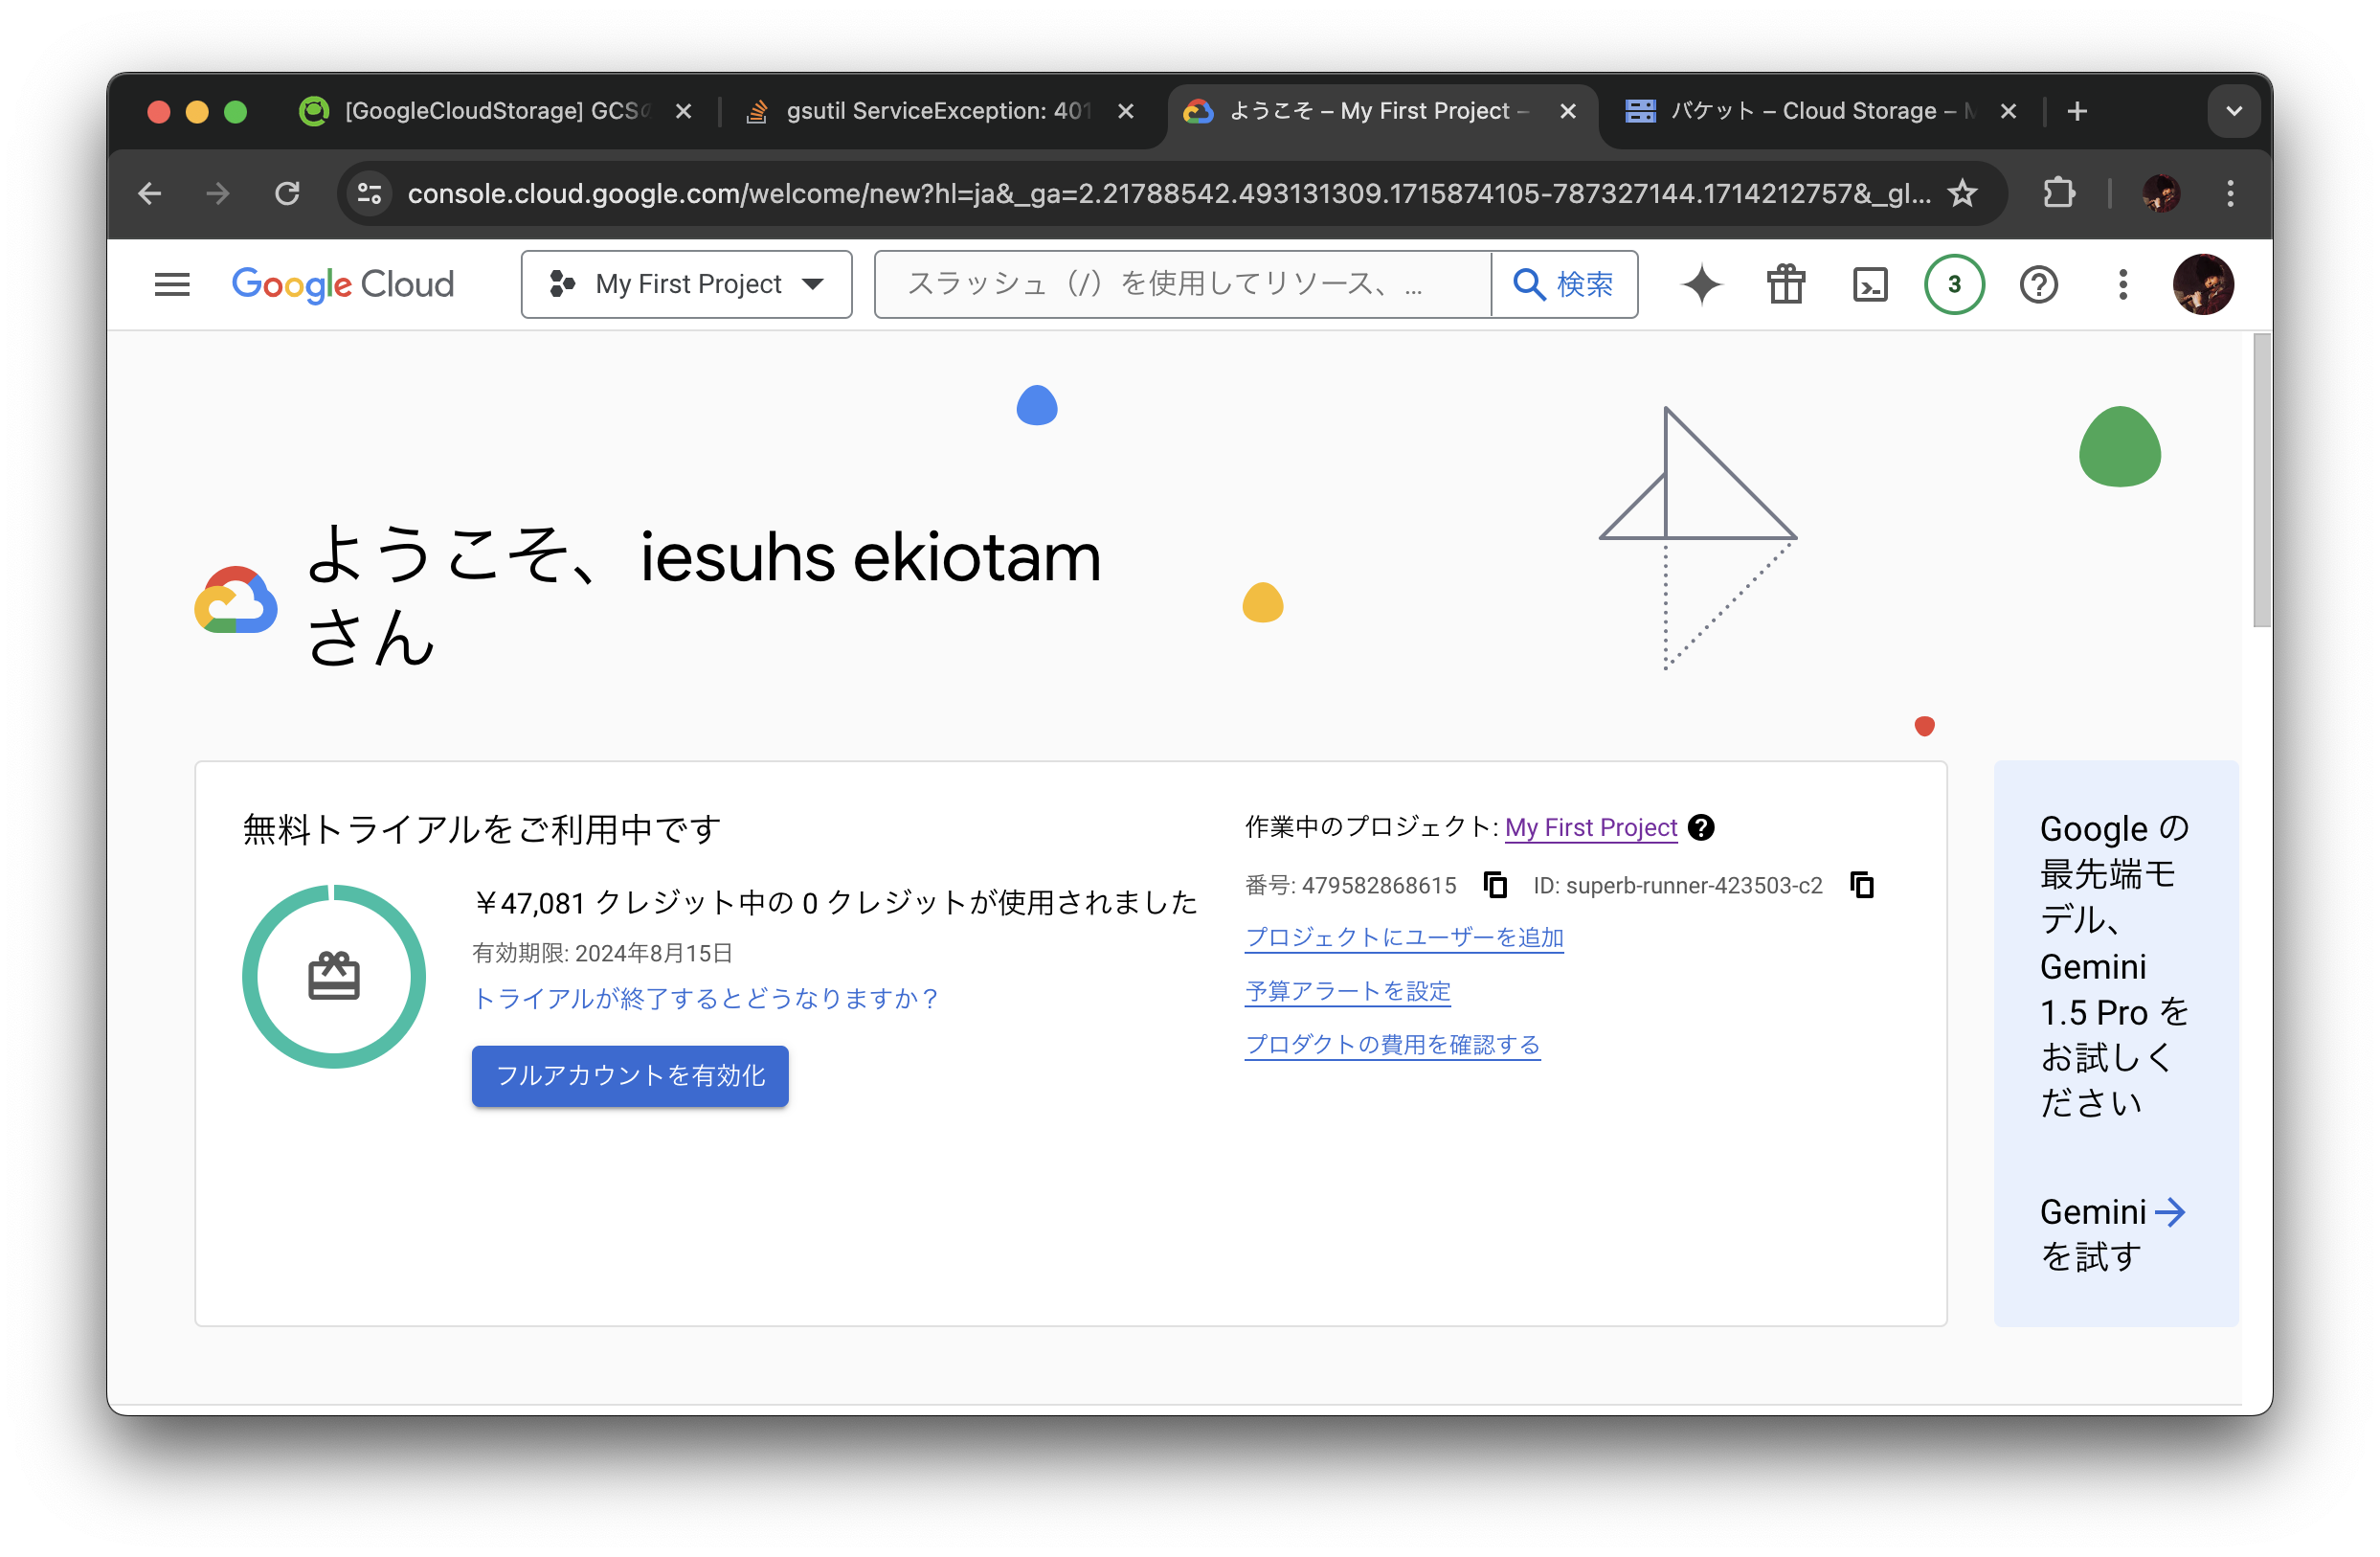
\includegraphics[keepaspectratio, scale=0.3]{figs/png/cloud1.png}
	
	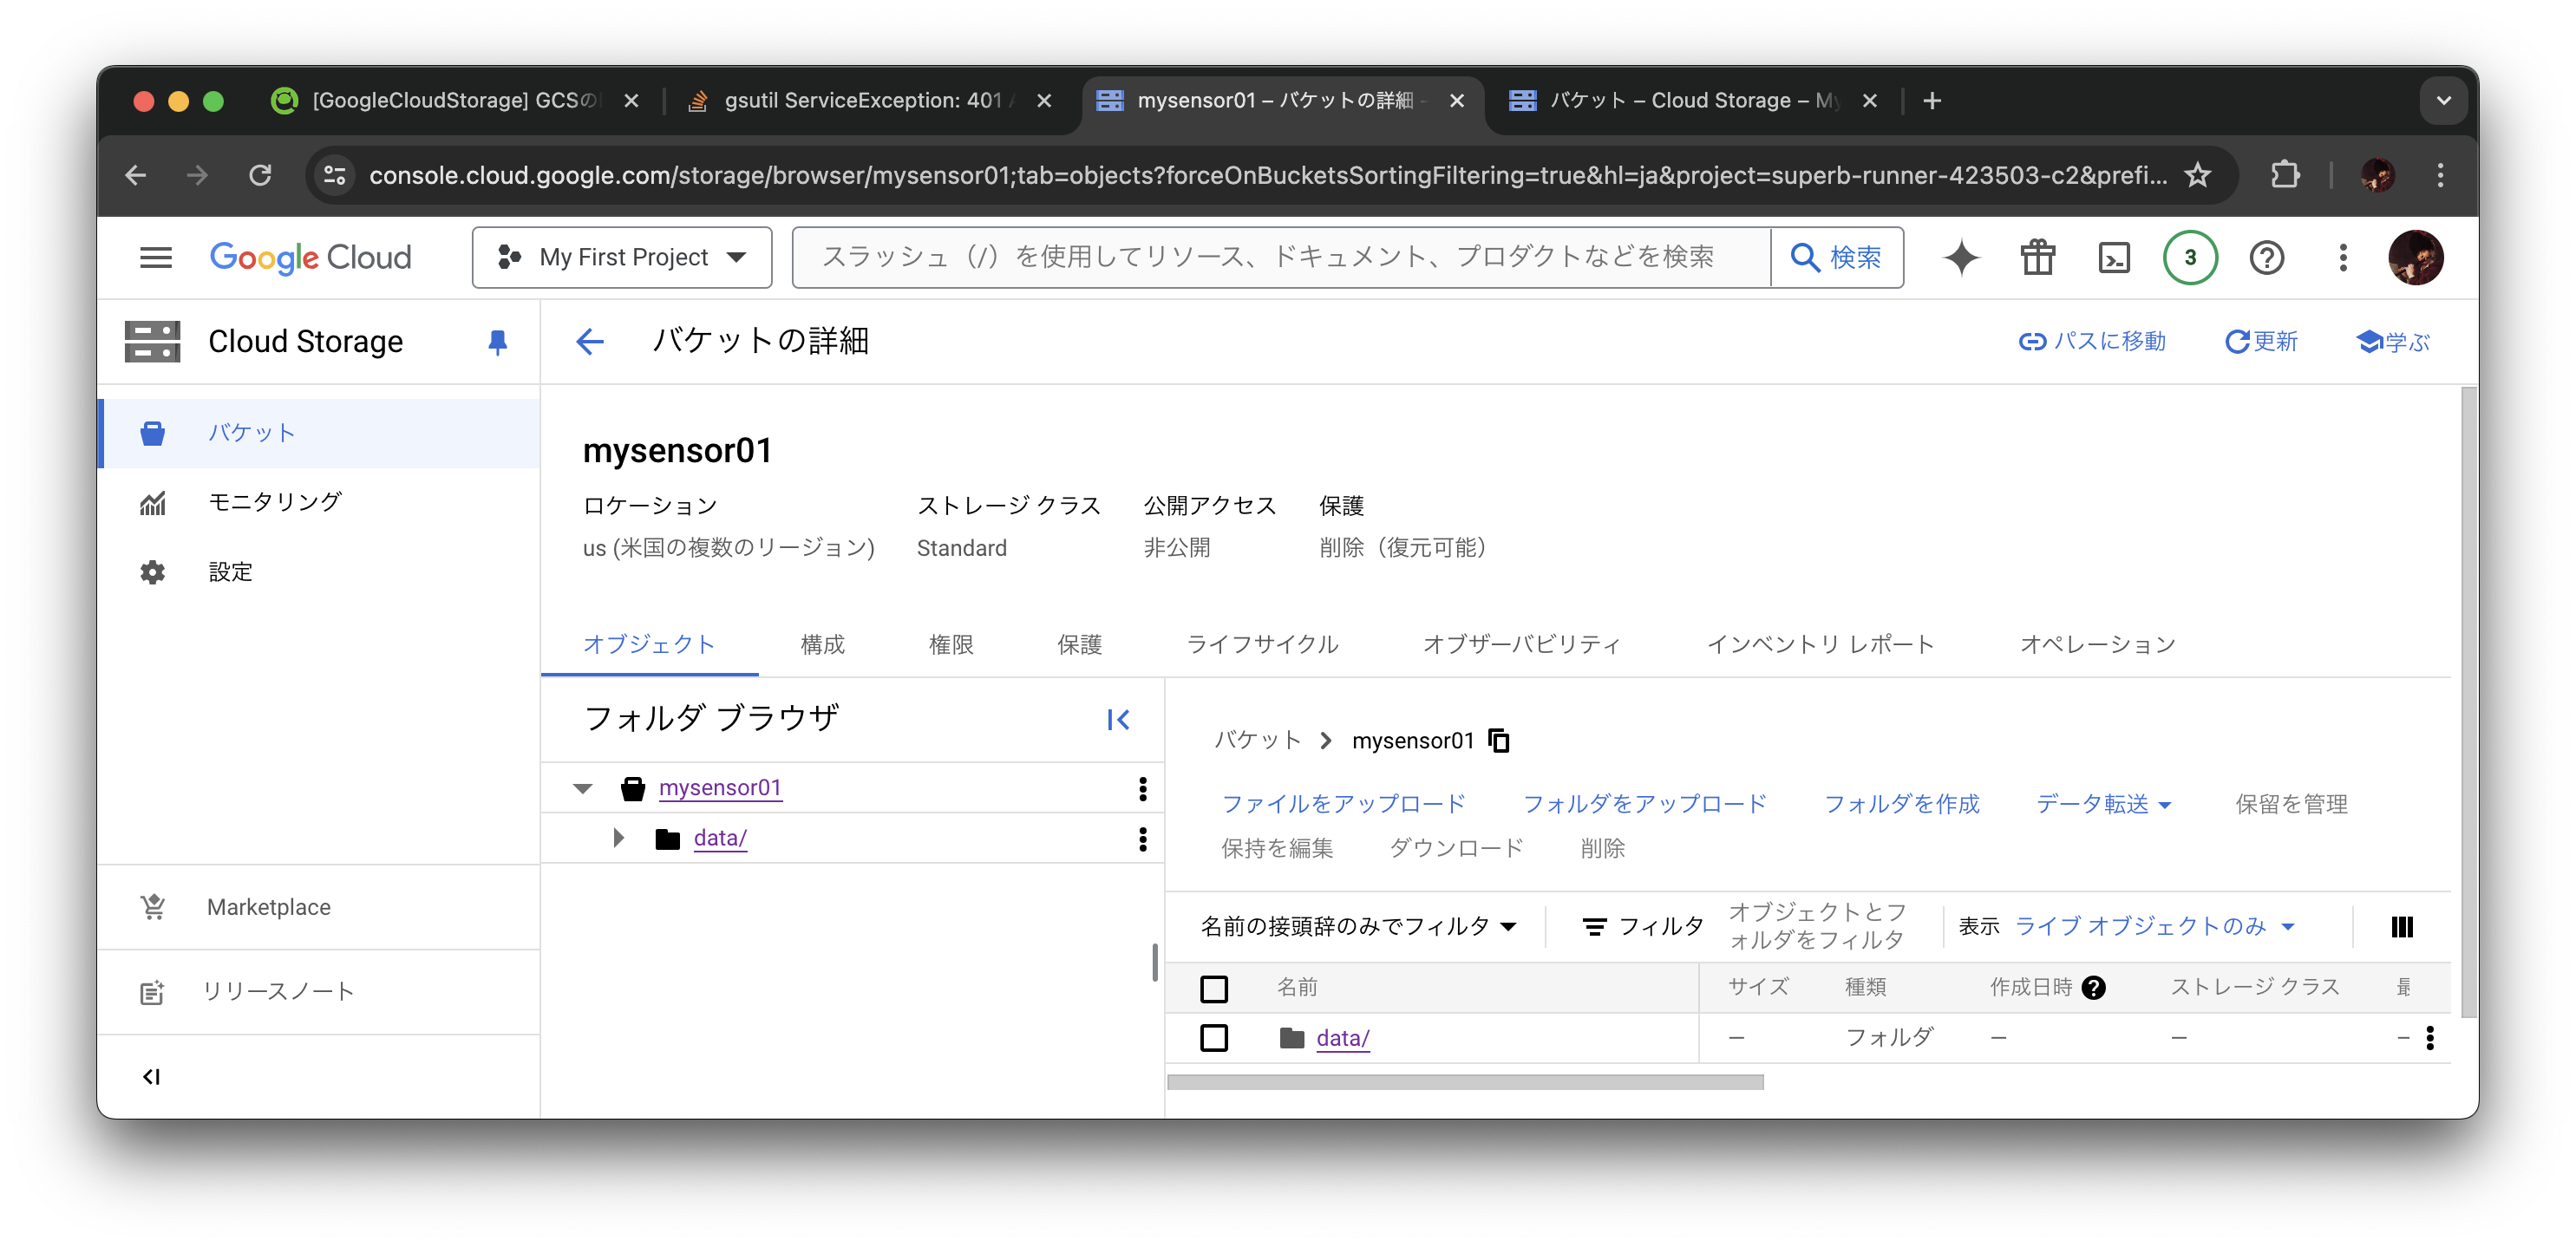
\includegraphics[keepaspectratio, scale=0.24]{figs/png/cloud2.png}
	
	\item プログラムからアクセスを試みると、アクセス権が無いという類のエラーに見舞われるので、Google Cloud CLI をインストール\footnote{\url{https://cloud.google.com/sdk/docs/install?hl=ja}}した後(ここ\footnote{\url{https://stackoverflow.com/questions/49302859/gsutil-serviceexception-401-anonymous-caller-does-not-have-storage-objects-list}}で議論されていることに従って)コマンドコンソールから次を行う(Yesを応答していく)
	\begin{verbatim}
		gcloud auth login
		gcloud auth application-default login
	\end{verbatim}
	
	プログラムで必要になるプロジェクト名は、WebUI上で作成した時の名前ではなく、application-default login の際、最後にコンソール上に表示されるものを使う必要がある
	
	\item ユーザ認証情報とサービス アカウント認証情報を上の手続きで提供できたなら、以下のjsonファイルに必要な情報が保存されているので、他のマシンでgoogle-cloud-storage のAPIを使用したプログラムを動かしたい場合、このjsonファイルを同じ場所にコピーして運用することができる
	\begin{verbatim}
		~/.config/gcloud/application_default_credentials.json
	\end{verbatim}
	
	\footnotetext[7]{\url{https://qiita.com/Hyperion13fleet/items/594c15ac24f149ab73c9}\label{fot:fn7}}
	もし、勝手な場所に保存したいなら、次の方法\footnotemark[7]もある様だ
	\begin{verbatim}
		from google.cloud import storage as gcs
		from google.oauth2 import service_account
		key_path = '{クレデンシャルを格納しているPath}'
		credential = service_account.Credentials.from_service_account_file(key_path)
		project_id = "{ProjectName}"
		client = gcs.Client(project_id, credentials=credential)
	\end{verbatim}
	
	\item 生成されたjsonファイルを読んでみると次の様になっている
	\begin{verbatim}
		{
			"account": "",
			"client_id": "764086051850-6h 途中略 di341hur.apps.googleusercontent.com",
			"client_secret": "d-FL95Q19q7MQmFpd7hHD0Ty",
			"quota_project_id": "superx-yrunner-123456-z2",
			"refresh_token": "1//0eF3EqrARA-9 途中略 3VL1aJ4ki3HIWdZT0H6YM-NKQ_rSw",
			"type": "authorized_user",
			"universe_domain": "googleapis.com"
		}
	\end{verbatim}
	プロジェクト名として指定するのに使うのは、"quota\_project\_id":の後に示されている文字列になる
	
	jsonファイルを読み書きするPythonのプログラムは次の通り
	\begin{spacing}{0.87}
	\begin{itembox}[l]{myjson.py}
		\begin{verbatim}
			import json
			
			#JSON ファイルの読み込み
			with open('application_default_credentials.json', 'r') as f:
			json_dict = json.load(f)
			print('json_dict:{}'.format(type(json_dict)))
			print(f'json_dict:\n{json_dict}')
			
			#JSON データの変換
			print('-----辞書型から JSON 形式の文字列へ変換-----')
			json_str = json.dumps(json_dict)
			print('json_str:{}'.format(type(json_str)))
			print(f'json_str:\n{json_str}')
			
			print('-----JSON 形式の文字列から辞書型へ変換-----')
			json_dict2 = json.loads(json_str)
			print('json_dict2:{}'.format(type(json_dict2)))
			print(f'json_dict2:\n{json_dict2}')
			
			#JSON データの書き込み
			with open('test2.json', 'w') as f2:
			json.dump(json_dict2, f2)
			with open('test2.json', 'r') as f3:
			f3_dict = json.load(f3)
			print(f'f3_dict:\n{f3_dict}')
		\end{verbatim}
	\end{itembox}
	\end{spacing}

	\item Pythonの仮想環境に次を導入しておく
	\begin{verbatim}
		pip install google-cloud-storage
		pip install gcsfs
		(以下は必要に応じて)
		pip install pillow
		pip install openpyxl
	\end{verbatim}
	
	\item GCS(google-cloud-storage)のPythonAPIは、以下のラッパークラス\footnotemark[7]を継承して利用させて頂くことにする(ありがたや)
	
	\setcounter{footnote}{7}
	
\end{enumerate}

\lstinputlisting[caption = GCSWrapper(gcloud.py), label = prog1]{src/local/gcloud.py}

このラッパークラスは、リモートマシンの日毎のデータをGCSにアップロードする際にも使っていた

以下は、GCSの操作\footnote{https://cloud.google.com/storage/docs/samples/?hl=ja}を試行したもの. 試しているのは、
\begin{itemize}
	\item テキストファイルのアップロードとダウンロード
	\item pandasのデータフレームのアップロードとダウンロード
	\item CSVファイルのアップロードとダウンロード
	\item GCS上のファイルの削除とファイル一覧の取得
\end{itemize}
なお、例えば data/ という名前のblobをアップロードするとフォルダができる

\newpage

\lstinputlisting[caption = check\_cloud.py, label = prog2]{src/local/check_cloud.py}

\section{新たなシステムへの移行の手順}

\subsection{ローカルマシンの移行}

ここまで作成してきたものを、新たなマシン(Raspberry Pi)へ移行する際、必要になる手続きについてまとめておく
(新しいマシンのOSが導入され、ネットワークの設定を終えた後の手続きになる)

\begin{figure}[htbp]
	\begin{minipage}[b]{1.0\linewidth}
		\centering
		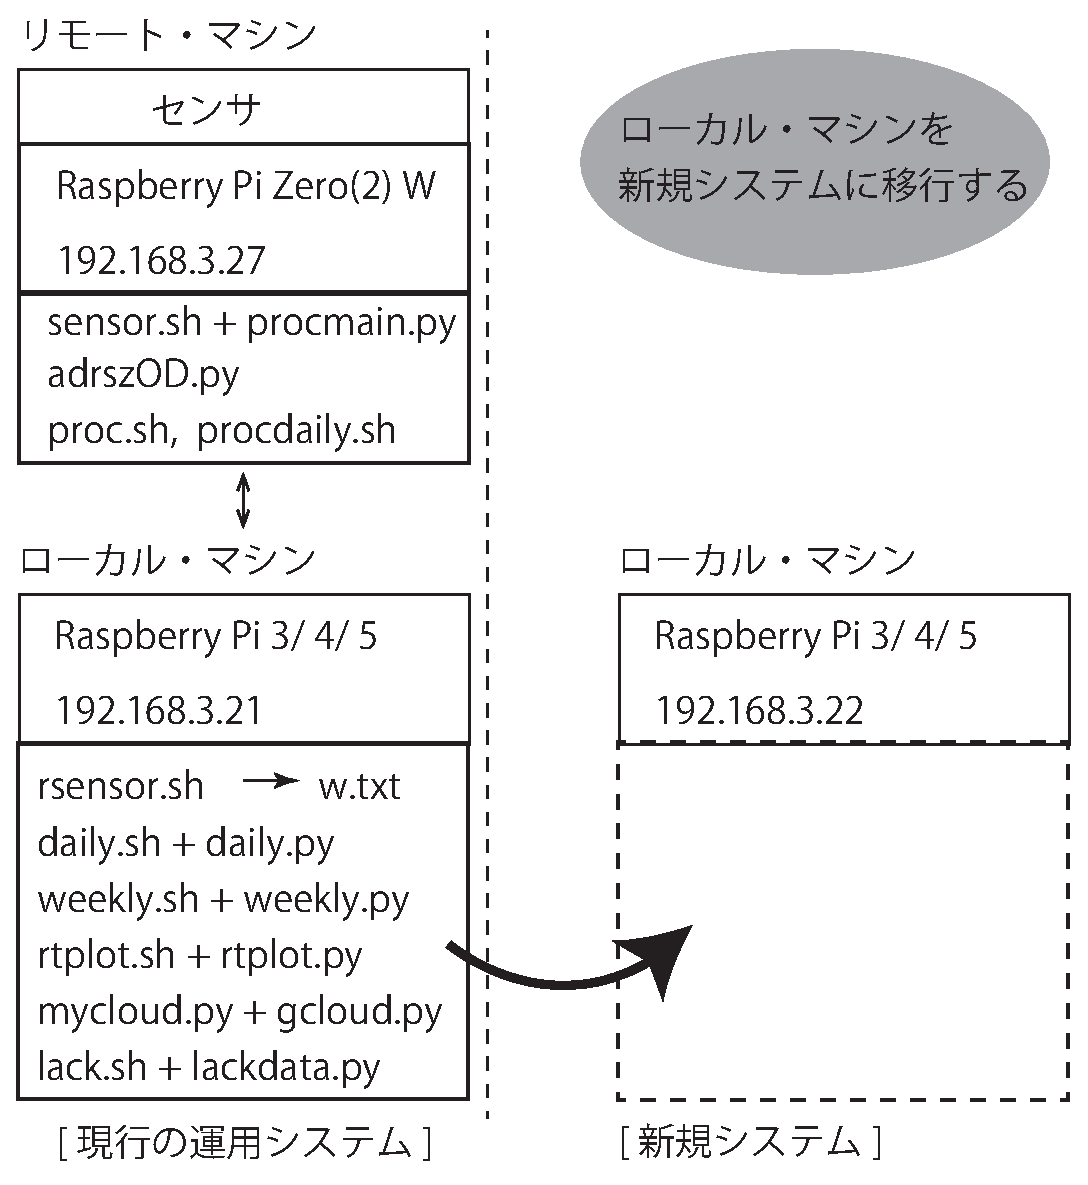
\includegraphics[keepaspectratio, scale=0.4]{figs/eps/ikou.eps}
		\caption{ローカルマシンの移行}
	\end{minipage}
	%\hspace{1.0cm}
	%\begin{minipage}[b]{0.45\linewidth}
	%\centering
	%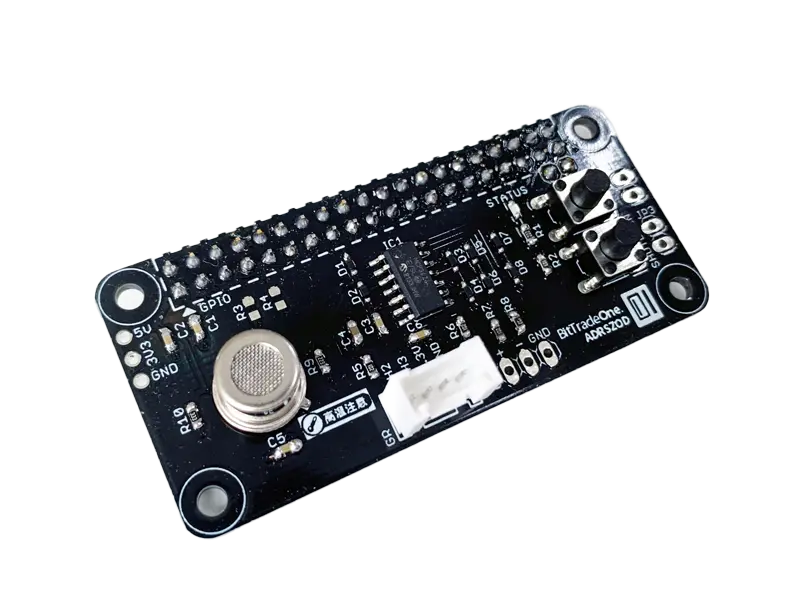
\includegraphics[keepaspectratio, scale=0.25]{figs/png/nioi_sensor.png}
	%\caption{ADRSZOD:TP401A}
	%\end{minipage}
\end{figure}

以下の手続きはその都度全て、/home/mat/Documents の直下で実施するものとする

\begin{enumerate}
	\item sshを有効にする(Raspberry Piのconfigulationで)
	\item システムを最新の状態にする
	\begin{verbatim}
		sudo apt update
		sudo apt dist-upgrade
	\end{verbatim}
	\item sshpass を導入する
	\begin{verbatim}
		sudo apt install -y sshpass 
	\end{verbatim}
	\item Pythonの仮想環境を /home/mat/Documents/venv11 につくる\footnote{寺田学 他3名、翔泳社「Pythonによるあたらしいデータ分析の教科書」第2版、p.50}
	\begin{verbatim}
		python3 -m venv venv11
		source venv11/bin/activate
		python3 -m pip install -U pip
		pip install numpy==1.22.4
		pip install scipy
		pip install pandas==1.4.2
		pip install matplotlib
		pip install scikit-learn
		pip list -o
		deactivate
	\end{verbatim}
	\item dataフォルダとfigsフォルダを移行する
	\begin{verbatim}
		scp -r mat@192.168.3.21:/home/mat/Documents/data ./
		scp -r mat@102.168.3.21:/home/mat/Documents/figs ./
	\end{verbatim}
	\item shellとPythonのプログラムを移行する
	\begin{verbatim}
		scp mat@192.168.3.21:/home/mat/Documents/*.sh ./
		scp mat@192.168.3.21:/home/mat/Documents/*.py ./
	\end{verbatim}
	ここで、各shellには実行可能属性がついている事を確認する ls -l *.sh\\
	もし付いていなかったら付ける chmod +x *.sh\\
	また、リモートマシンのIPアドレス、ユーザ名とそのパスワードが変わる場合は、ここで rsensor.sh の当該箇所(露に記述している)を編集する\\
	Pythonのプログラムに実行可能属性は不要である
	\item cronに時刻指定手続きを登録する(crontab -e)
	\begin{verbatim}
		MAILTO=""
		*/5 * * * * sh /home/mat/Documents/rsensor.sh
		56 23 * * * sh /home/mat/Documents/daily.sh
		1 0 * * Sun sh /home/mat/Documents/weekly.sh
	\end{verbatim}
	\item sshでリモートマシンに接続を試みて、key fingerprint を登録させる
	\begin{verbatim}
		ssh mat@192.168.3.27
		 The authenticity of host '192.168.3.27' can't be established.
		 ED25519 key fingerprint is SHA256:......
		 This key is not known by any other names.
		 Are you sure you want to continue connecting (yes/no/[fingerprint])? yes
		ssh mat@192.168.3.27 /home/mat/Documents/sensor.sh
	\end{verbatim}
	\item txtファイルを移行する
	\begin{verbatim}
		scp mat@192.168.3.21:/home/mat/Documents/*.txt ./
	\end{verbatim}
	\item rsensor.sh が5分ごとに起動され、w.txt を更新している事を確認する
	\begin{verbatim}
		tail -f w.txt
	\end{verbatim}
	\item 実時間モニタ用のプログラムを起動する
	\begin{verbatim}
		source venv11/bin/activate
		python3 ./rtplot.py
	\end{verbatim}
\end{enumerate}

\subsection{リモートマシンの移行}

新しいリモートマシンへの移行は次の通り\\リモートマシンへのOSの導入とネットワークの設定を終えていること

\begin{enumerate}
	\item configurationで、sshとi2cを有効にする
	\item 最新の状態に更新する
	\begin{verbatim}
		sudo apt update
		sudo apt dist-upgrade
	\end{verbatim}
	\item adrszOD.py と procmain.py、及び proc.sh、procdaily.sh を導入する
	\item sensor.sh を導入して、実行可能属性をつける(chmod +x sensor.sh)
	\item /home/mat/Documents/sensor.sh を実行して、現在日時とセンサの電圧、それぞれ適切な値が1行で出力される事を確認する
\end{enumerate}


\begin{thebibliography}{99}
	\bibitem{1} ビット・トレード・ワン社zerooneシリーズ拡張基板のサンプルプログラム\\
	(\url{https://github.com/bit-trade-one/RasPi-Zero-One-Series})
	\bibitem{2} BME280センサーモジュール\\
	(\url{https://algorithm.joho.info/programming/python/raspberrypi3-bme280-kion-sitsudo-kiatsu/})
	\bibitem{3} matplotlib が認識する日付の書式\\
	(\url{https://matplotlib.org/stable/api/dates_api.html})
	\bibitem{4} テキストの結合、プロセス置換\\
	Daniel J.Barrett著、オライリー・ジャパン「Efficient Linuxコマンドライン」初版第1刷、p.106(テキストの結合), p.154, p.157 のコラム記事
	\bibitem{5} Pythonの仮想環境\\
	寺田学 他著、翔泳社「Pythonによるあたらしいデータ分析の教科書」第2版、p.50
	\bibitem{6} 「source」コマンドと「.」コマンド\\
	(\url{https://atmarkit.itmedia.co.jp/ait/articles/1712/21/news015.html})
	\bibitem{7} Google Cloud Console -> Cloud Storage\\
	(\url{https://console.cloud.google.com/welcome/new?hl=ja})
	\bibitem{8} Wrapper class for Python API of Google Cloud Storage\\
	(\url{https://qiita.com/Hyperion13fleet/items/594c15ac24f149ab73c9})
	\bibitem{9} Google Cloud CLI\\
	(\url{https://cloud.google.com/sdk/docs/install?hl=ja})\\
	(\url{https://stackoverflow.com/questions/49302859/gsutil-serviceexception-401-anonymous-caller-does-not-have-storage-objects-list})
	\bibitem{10} Code samples with GCS API\\
	(\url{https://cloud.google.com/storage/docs/samples/?hl=ja})
	\bibitem{11} gcsfs
	(\url{https://dodotechno.com/python-gcs/})
\end{thebibliography}

\end{document}          
